\documentclass[12pt]{report}

\usepackage[utf8]{inputenc}
\usepackage{graphicx}
\usepackage[backend=bibtex, sorting=none]{biblatex}
\usepackage{amsmath}
\usepackage{gensymb}
\usepackage[italian]{babel}
\usepackage[toc, page]{appendix}
\usepackage{hyperref}
\usepackage{caption}
\usepackage{float}
\usepackage{listings}
\usepackage{tabularx}
\usepackage{enumerate}
\usepackage{markdown}
\usepackage{subcaption}

\nocite{*}
\addbibresource{riferimenti.bib}
\graphicspath{{images/}}

\title{
	Analisi Time Series\\
	\large Progetto di Data Science e Machine Learning
}
\author{De Stefano Manuel, Esposito Flavio, Iannone Emanuele}
\date{Luglio 2019}

\begin{document}
\maketitle
\tableofcontents

\chapter{Introduzione} \label{chap:intro}
\section{Il contesto}
Una \textbf{time series}\footnote{Nel seguito verrà usato anche \textit{TS}} (serie temporale) è una serie di dati ordinati nel tempo. Tipicamente, i dati sono presi ad intervalli di tempo regolari. Alcuni esempi sono gli elettrocardiogrammi, l'andamento delle maree, i valori azionari.
\begin{figure}[H]
	\centering
	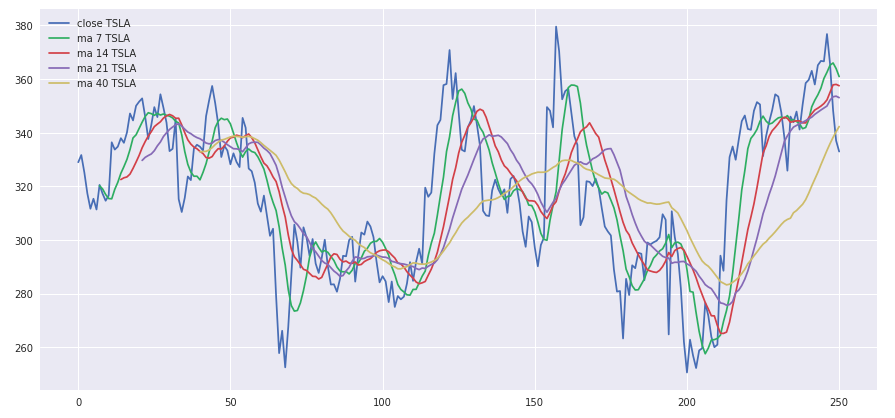
\includegraphics[width=\linewidth]{timeseries.png}
	\caption{Un'insieme di TS, ciascuna di colore diverso}
	\label{fig:timeseries}
\end{figure}
Le TS, quindi, sono molti simili a dei segnali, quindi analizzabili sia in dominio del tempo che in dominio della frequenza.\\
\\
L'\textbf{analisi di time series} si occupa di analizzare questi dati per estrarre informazioni statisticamente rilevanti per diversi scopi:
\begin{itemize}
	\item \textbf{Previsioni}, per prevedere andamento di alcuni eventi nel futuro, come le azioni in borsa, oscillazioni della terra, tramite un modello statistico;
	\item \textbf{Stime}, per approssimare l'informazione portata da segnali di vario genere;
	\item \textbf{Anomaly detection}, per identificare alcuni pattern ricorrenti sospetti.
\end{itemize}
Per portare a termine questi scopi, i principali task sulle TS sono:
\begin{itemize}
	\item \textbf{Classificazione}, che consiste nella costruzione di un modello che apprende dai dati (le TS) il modo in cui assegnare a ciascuna di loro una label. Il modello può essere basato su SVM, k-NN, reti neurali, regressione o alberi di decisione. L'apprendimento è di tipo supervisionato, quindi sono necessarie delle label assegnate ai dati di addestramento;
	\item \textbf{Clustering}, che consiste nel partizionare un insieme di TS a seconda della loro similarità. Bisogna dapprima scegliere una metrica di similarità (o distanza), come può essere la distanza Euclidea o la tecnica del DTW\footnote{Dynamic Time Warping}, e poi un algoritmo di clustering, come può essere k-Means o DBSCAN. L'apprendimento è di tipo non supervisionato, quindi non sono necessarie delle label assegnate ai dati di addestramento.
\end{itemize}
Analizzare le TS, a differenza dell'analisi di altri tipi di dati, presenta qualche difficoltà:
\begin{itemize}
	\item Ogni singola misurazione della TS è memorizzata in una colonna del dataset, quindi TS con un \textbf{alto numero di misurazioni} comporta un forte aumento della sua dimensionalità, rendendo lunga la sua fase di training e creando modelli non performanti\footnote{Questo problema è noto come \textbf{curse of dimensionality}};
	\item E' difficile trovare una metrica di similarità che sia \textit{valida}, ovvero che ritorni un valore alto di similarità per le sole TS effettivamente simili, ed \textit{efficiente}, ovvero che il suo tempo di calcolo sia accettabile;
	\item Alcune TS di una certa tipologia potrebbero essere di \textbf{lunghezza differente}, andando a danneggiare di molto le performance del modello.
\end{itemize}
Per risolvere il problema della dimensionalità bisognerebbe usare tecniche di \textbf{feature extraction and selection}, in modo tale da far allenare i modelli su un insieme ridotto di feature rilevanti oppure trasformare l'input (la singola TS) in un "formato ridotto" che ne preserva le caratteristiche.\\
Per risolvere il problema della metrica di similarità bisognerebbe ricorrere a delle funzioni di distanza che tengono conto della natura delle TS.\\
E' possibile risolvere il problema della lunghezza usando opportune tecniche di feature selection oppure metriche di similarità ad hoc per le TS.

\section{Il problema}
Si vuole compiere del \textbf{clustering} di alcuni dataset di TS al fine di \textbf{accomunare quelle simili}.\\
Le TS potrebbero portare con sè delle label rappresentanti la loro classe di appartenenza, da ignorare ai fini del clustering in sè, essendo l'apprendimento di tipo non supervisionato. Esse, saranno comunque usate per validare esternamente i risultati ottenuti dall'algoritmo di clustering.\\
Inoltre, si vuole che ciascun dataset possieda solo TS di lunghezza uguale.

\section{Stato dell'arte}
L'analisi delle time series è uno studio abbastanza diffuso e in letteratura esistono diversi lavori che hanno dato un importante contributo.\\
\\
\textbf{TSFresh}\cite{tsfresh} è una libreria per Python, compatibile con Scikit-Learn, per l'estrazione automatica di feature di time series, ovvero caratteristiche rilevanti delle stesse, come la media, il valore minimo, il numero di picchi, la mediana, ecc. La libreria è anche in grado di assegnare un \textit{valore di rilevanza} alle feature, così da permetterne una selezione delle sole rilevanti. Viene offerto anche un supporto al calcolo parallelo e distribuito.\\
L'estrazione e selezione delle feature sono un aspetto cruciale nell'analisi delle TS poiché esse permetteno la riduzione della loro dimensionalità, rendendole quindi trattabili.\\
TSFresh non fornisce alcun modello di classificazione, regressione o clustering, quindi non si sostituisce ad altre librerie di machine learning come Scikit-Learn.\\
\\
\textbf{TSLearn}\cite{tslearn} è una libreria per Python scritta in C++ per l'analisi di time series. A differenza di TSFresh, essa offre, tra l'altro, dei modelli di apprendimento ad hoc per le TS. E' in grado di leggere i dataset, di farne del preprocessing, di compiere classificazione e regressione con SVM e clustering, usando metriche di distanza ad hoc per le TS, come il DTW.\\
Tuttavia, rispetto a TSFresh, è meno matura: ha pochi algoritmi implementati, una documentazione meno ricca, meno contributors e fork.

\section{Soluzione proposta}
Per affrontare il problema descritto si farà uso di un \textbf{autoencoder}, una particolare rete neurale in grado di fornire una rappresentazioni compatta dei suoi input (qui le TS), detta \textbf{vettore latente}, di dimensione ridotta e decisa tramite iperparametri del modello.\\
DESCRIZIONE BREVE EXTRA\\
Sui vettori latenti del test set verrà lanciato il clustering con k-Means, reiterato più volte per una maggiore stabilità e con un diverso numero di cluster.\\
\\
Per realizzare queste soluzioni è stato scelto il linguaggio \textit{Python} per via dell'alto supporto fornito dalle sue libreria, quali \textit{Scikit-Learn}\cite{sklearn_api}, \textit{NumPy}\cite{numpy}, \textit{Matplotlib}\cite{matplotlib} e \textit{Pandas}\cite{pandas}. Il codice è stato inserito in notebook \textit{Jupyter}, così da poter visualizzare subito i risultati di alcuni snipper di codice, di rieseguirli velocemente e di immergere anche dei commenti in \textit{Markdown}.\\

\section{Validazione della soluzione}
Per poter valutare le prestazioni dell'autoencoder si adotteranno alcune misure interne e misure esterne\cite{metrics} di clustering. Esse, oltre a stabilire la qualità dell'algoritmo di clustering in sè, servono anche per trovare il numero di cluster ottimale nel caso in cui l'algoritmo non è in grado di stabilirlo da sè, come nel caso di k-Means.\\
\\
I risultati del modello verranno confrontati con quelli ritornati dal k-Means con metrica di distanza DTW offerto dalla libreria TSLearn. Questo confronto serve a stabilire quanto è affidabile questo modello sui dataset in esame.\\
Inoltre, i risultati del modello saranno confrontati con altri lavori simili.

\subsection{Misure di validazione interne}
Una \textbf{misura di validazione interna} si occupa di validare i risultati di un algoritmo di clustering guardando quanto bene ha accomunato (messi in uno stesso cluster) item simili e quanto bene ha separato (messi in cluster diversi) item diversi.\\
In altre parole, si vuole minimizzare la distanza intra-cluster e massimizzare la distanza inter-cluster\footnote{Questa distanza è calcolata a seconda della metrica di distanza scelta}.\\
\\
La \textbf{compactness} (o cohesion) misura quanto bene sono vicini gli item in ciascun cluster ed è, tipicamente, la somma dei quadrati di tutte le distanze degli item di un cluster dal relativo centroide. E' bene minimizzarla il più possibile.\\
La \textbf{separation} misura quanto bene sono distanziati gli item in diversi cluster ed è, tipicamente, la somma dei quadrati di tutte le distanze tra tutti i centroidi. E' bene massimizzarla il più possibile.\\
Una misura di validazione tiene conto sia della compactness che della separation in qualche modo.\\
\\
E' bene ricordare che alcuni algoritmi di clustering già hanno come scopo quello di ottimizzare compactness e/o separation, quindi potrebbe capitare che alcuni indici risultino quasi sempre alti, diventando meno rilevanti in quel caso.

\subsubsection{Silhouette Coefficient}
Il \textbf{Silhouette Coefficient di un item $i$} serve a stabilire quanto bene $i$ è stato assegnato al giusto cluster.\\
\\
Sia $i$ un'item e sia $d$ una qualsiasi funzione di distanza. Il Silhouette Coefficient di i, $S(i)$ si calcola nel seguente modo:
\begin{align}
S(i) = \frac{b_i - a_i}{max(a_i, b_i)}
\end{align}
dove:
\begin{enumerate}[(i)]
	\item $$ a_i = \frac{1}{|C|-1}\sum_{i\ne j\in C} d(i,j)$$ è la distanza media dell'item i rispetto agli altri item j nello stesso cluster C.\\
	Più il valore è piccolo, più l'item i è vicino agli altri item dello stesso cluster;
	\item $$ b_i = \min_{k\ne i} \frac{1}{|C_k|}\sum_{j \in C_k} d(i,j)$$ è la distanza media dell'item i rispetto agli item j nel più vicino cluster\footnote{Anche detto \textit{neighbour cluster}} diverso da quello che contiene i.
\end{enumerate}
E' compreso tra -1 e 1, con -1 indicante un clustering totalmente errato, 1 indicante un clustering altamente denso e ben separato e 0 indicante clustering sovrapposti.\\
Si osserva che se $b_i > a_i$, allora $S(i)$ risulterà compreso tra -1 e 0, sintomo di un'assegnazione di i al cluster sbagliato: sarebbe più opportuno assegnarlo al cluster più vicino.\\
Se $b_i < a_i$, allora $S(i)$ risulterà compreso tra 0 e 1. Più $a_i$ tende a 0, più $S(i)$ tenderà ad 1, sintomo di perfetta assegnazione di i al cluster giusto.\\
Se $S(i)$ è circa 0 allora l'item non dovrebbe stare in nessuno dei due cluster proposti, e sarebbe quindi opportuno rivalutare il numero di cluster scelti, se non proprio l'algoritmo di clustering stesso.\\
\\
E' possibile calcolare il Silhouette Coefficient medio di tutto il clustering. Sia D l'insieme di tutti gli item:
\begin{align}
S = \frac{1}{|D|} \sum_{i \in D} S(i)
\end{align}
Più S tende ad 1, migliore è l'assegnazione degli item.\\
La sua elaborazione può richiedere molto tempo se la metrica di distanza è complessa.

\subsubsection{Dunn Index}
Il \textbf{Dunn Index} di un clustering misura quanto bene i cluster sono compatti e separati l'uno dall'altro.\\
\\
Sia m il numero di cluster, il Dunn Index è calcolabile nel seguente modo:
\begin{align}
D = \frac{\min_{1\le i \le j \le m}\delta(C_i, C_j)}{\max_{1 \le k \le m}(diam(C_k))}
\end{align}
dove:
\begin{enumerate}[(i)]
	\item $ \delta(C_i, C_j) $ è la separation tra due cluster $C_i$ e $C_j$, calcolata attraverso una qualsiasi metrica di distanza.\\
	Il numeratore di D considera la più piccola di queste separazioni, escludendo quelle già calcolate;
	\item $ diam(C_k) $ è una funzione che calcola il \textit{diametro} del cluster $C_k$, ovvero la massima distanza (di qualsiasi tipo) tra due dei suoi item. E' una particolare misura di compactness.
\end{enumerate}
Cluster molto grandi hanno una maggiore probabilità di avere un diametro maggiore, e quindi una maggiore probabilità di aumentare il denominatore di $D$, andando a diminuire l'indice. Aumentare di molto il numero di cluster andrà ad aumentare $D$ con alta probabilità.\\
E' un indice rilevante in dataset molto grandi e/o quando è previsto avere un grande numero di cluster.

\subsubsection{Davies-Bouldin Index}
Il \textbf{Davies-Bouldin Index} di un clustering misura la media di similarità di ciascun cluster con il suo cluster più simile.\\
\\
Sia m il numero di cluster, il Davies-Bouldin Index è calcolabile nel seguente modo:
\begin{align}
DB = \frac{1}{m}\sum_{i=1}^{m}\max_{i \ne j}sim(C_i, C_j)
\end{align}
dove:
\begin{enumerate}[(i)]
	\item $$ sim(C_i, C_j) =  \frac{c_i + c_j}{d(C_i, C_j)}$$ è una misura di \textit{similarità tra due cluster}.\\
	$c_i$ è la compactness del cluster $C_i$ calcolata come distanza media di tutti gli item in $C_i$ rispetto al proprio centroide.\\
	$d(C_i, C_j)$ è la separation tra i cluster $C_i$ e $C_j$, calcolata come distanza tra i rispettivi centroidi.
\end{enumerate}
Ha 0 come lower bound, e a differenza di altri indici un buon clustering è rappresentato da un DB tendente a 0. Per minimizzare DB, bisogna rendere i cluster il meno simile possibile, realizzabile minimizzando le compactness di ciascun cluster (i valori $c_i$) oppure massimizzando la separation tra cluster ($d(C_i, C_j)$).\\
Cluster molto densi e distanti hanno DB minimo. Con DBSCAN si raggiungono quasi sempre score tendenti a 0 poiché è l'algoritmo stesso che ottimizza la densità dei cluster.

\subsection{Misure di validazione esterne}
Una \textbf{misura di validazione interna} si occupa di validare i risultati di un algoritmo di clustering rispetto a delle \textbf{ground truth}\footnote{Verità di base}, ovvero delle informazioni relative ad un altro tipo di clustering o classificazione degli stessi dati non usate per compiere il clustering in esame.\\
Nelle ground truth, quindi, \textbf{ogni item possiede una classe} (o label), da usare come oracolo.\\
\\
A differenza delle misure interne, che si pongono di misurare cluster compatti e separati, le misure esterne si occupano di misurare cluster \textit{fedeli} a delle ground truth. La fedeltà è spesso misurata tramite \textbf{pair counting}\footnote{Conteggio delle coppie}, ovvero contando:
\begin{itemize}
	\item Il numero di coppie di item clusterizzati insieme se essi sono della stessa classe. Anche detto numero di \textbf{True Positive} (TP);
	\item Il numero di coppie di item clusterizzati insieme se essi sono in classi diverse. Anche detto numero di \textbf{False Positive} (FP);
	\item Il numero di coppie di item NON clusterizzati insieme se essi sono della stessa classe. Anche detto numero di \textbf{False Negative} (FN);
	\item Il numero di coppie di item NON clusterizzati insieme se essi sono in classi diverse. Anche detto numero di \textbf{True Negative} (TN);
\end{itemize}
Chiaramente, come nel task della classificazione, lo scopo generale è quello di massimizzare TP e TN e di minimizzare FP e FN.

\subsubsection{Contingency Matrix}
La \textbf{Contingency Matrix} riporta la cardinalità delle intersezioni dei cluster con le classi delle ground truth. L'elemento $x_{ij}$ rappresenta il numero di item della classe i presenti nel cluster j.\\
Quanti più valori tendenti a 0 ha una colonna, più quel cluster è fedele ad una delle classi. Se il numero di cluster è uguale al numero di classi, è bene che un cluster ne ricopra una e una sola.\\
\begin{table}[H]
	\centering
	\begin{tabular}{l | l l l l}
		& $A_1$ & $A_2$ & $...$ & $A_m$\\
		\hline
		$B_1$ & $x_{11}$ & $x_{12}$ & $...$ & $x_{1m}$\\
		$B_2$& $x_{21}$ & $x_{22}$ & $...$ & $x_{2m}$\\
		$...$ & $...$ & $...$ & $...$ & $...$\\
		$B_n$& $x_{n1}$ & $x_{n2}$ & $...$ & $x_{nm}$
	\end{tabular}
	\caption{Contingency Matrix che confronta un labelling di n classi e un clustering di m cluster. $x_{ij}$ è il numero di item della classe i presenti nel cluster j}
	\label{tab:contingency}
\end{table} 
Non essendo un singolo valore, risulta di difficile interpretazione se il numero di cluster/classi aumenta. Allo stesso tempo, è molto utile per dare una prima interpretazione della fedeltà del clustering rispetto alle ground truth.

\subsubsection{Purity}
La \textbf{Purity} è una misura che stabilisce quanto bene un clustering copra un labelling/clustering di riferimento. Precisamente, misura quanto un cluster contiene elementi di una singola classe.\\
\\
Formalmente, sia C il clustering analizzato, L l'insieme di classi di riferimento, e sia N l'insieme degli item:
\begin{align}
P = \frac{1}{|N|}\sum_{c \in C}\max_{l \in L}|c \cap l|
\end{align}
E' compresa tra 0 e 1, con 0 indicante nessuna copertura, e 1 indicante copertura massima.\\
Ogni cluster partecipa alla sommatoria con il numero di item della classe assolutamente più diffusa al suo interno. Guardando alla Contingency Matrix, si sommano i valori massimi di ciascuna colonna.\\
\\
Non è consigliata con classi sbilanciate poiché risulterà facilmente alta per via dell'alta probabilità che un cluster abbia come classe più diffusa quella massima.\\
Per ridurre questo effetto negativo si potrebbe pensare di considerare il massimo relativo di ciascun cluster invece che del massimo assoluto: ogni cluster partecipa alla sommatoria con il numero di item della classe relativamente più diffusa al suo interno.\\
La divisione viene comunque fatta sul numero totale di elementi. Questa misura può essere chiamata \textbf{Purity Relativa}, anche essa compresa tra 0 e 1 e con uguale significato.

\subsubsection{Rand Index e Adjusted Rand Index}
Il \textbf{Rand index}, o \textbf{Accuracy}, è il rapporto tra il numero di coppie correttamente clusterizzate (ottenuto dalla somma di TP e TN) sul numero di coppie non ordinate totali.\\
Sia n il numero di item, il Rand Index si calcola nel seguente modo:
\begin{align}
RI = \frac{TP + TN}{C_2^n}
\end{align}
Il numero di coppie non ordinate può anche essere calcolato sommando TP, FP, FN e TN.\\
E' compreso tra 0 e 1, dove 0 indica che il clustering e il labelling non concordano su alcun punto, mentre 1 indica che c'è concordanza massima.\\
\\
Il Rand Index presenta un problema grave: valutare un \textit{clustering casuale uniforme}, anche detto \textbf{random labelling}, rispetto ad ground truth determina un buon valore, crescente con il numero di cluster creati. Chiaramente questa situazione non è desiderabile, ed è casuata dal fatto che i quattro valori incidono tutti allo stesso modo sul risultato.\\
Per risolvere questo problema si usa una versione "aggiustata" dell'indice, chiamata \textbf{Adjusted Rand Index} (ARI)\cite{ari}.\\
L'ARI tiene conto del RI del random labelling e lo usa come riferimento:
\begin{align}
ARI = \frac{RI - E[RI]}{max(RI) - E[RI]}
\end{align}
dove:
\begin{enumerate}[(i)]
	\item $ RI $ è il Rand Index calcolato al solito modo;
	\item $ E[RI] $ è il valore atteso del Rand Index, calcolabile con la formula del valore atteso di una variabile aleatoria ipergeometrica (il Rand Index può essere modellato come ipergeometrica) oppure calcolando il RI di un clustering uniforme casuale;
	\item $ max(RI) $ è il massimo valore che può assumere il Rand Index, calcolato come media del numero di coppie di item di ciascun cluster e di ciascuna classe.
\end{enumerate}
E' compreso tra 1- e 1, dove -1 indica che il clustering è come se fosse casuale rispetto al labelling, mentre 1 indica match perfetto.\\

\subsubsection{Pairwise Precision, Recall, F1-Score e Fowlkes-Mallows Index}
Precision, Recall ed F1-Score sono misure molto usate nel task di classificazione, e possono riproposte anche nel clustering se considerate nella loro versione pairwise, cioè che contano il numero di coppie invece che i singoli item.\\
La \textbf{Precision} di un clustering rispetto a delle ground truth è calcolata nel seguente modo:
\begin{align}
Pr = \frac{TP}{TP + FP}
\end{align}
La \textbf{Recall} di un clustering rispetto a delle ground truth è calcolata nel seguente modo:
\begin{align}
Re = \frac{TP}{TP + FN}
\end{align}
L'\textbf{F1-Score} di un clustering rispetto a delle ground truth è la media armonica di Precision e Recall; calcolata nel seguente modo:
\begin{align}
F_1 = 2\:\frac{Pr * Re}{Pr + Re}
\end{align}
Il \textbf{Fowlkes-Mallows Index}, o \textbf{G-Measure} di un clustering rispetto a delle ground truth è la media geometrica di Precision e Recall; calcolato nel seguente modo:
\begin{align}
FM = \sqrt{Pr * Re}
\end{align}
Tutte e quattro le misure sono comprese tra 0 e 1, con 0 indicante totale indipendenza tra clustering e labelling, e con 1 indicante match perfetto.\\
Il Fowlkes-Mallows è immune al random labelling: in quel caso ritorna uno score tendente a 0.\\
Nessuna delle quattro misure tiene conto dei TN, cosa che potrebbe essere utile in alcuni casi.

\subsubsection{Altre misure}
Esistono numerose altre misure esterne, tra le quali:
\begin{itemize}
	\item \textbf{Homogeneity}, misura quanto un cluster contenga item di una singola classe;
	\item \textbf{Completeness}, misura quanto gli item di una classe appartengano allo stesso cluster;
	\item \textbf{V-Measure}, media armonica tra Homogeneity e Completeness. Non è immune al random labelling;
	\item \textbf{Jaccard Index}, basata sulla similarità di Jaccard che è il rapporto tra TP e la somma di TP, FP e FN;
	\item \textbf{Dice Index}, come il Jaccard, ma da un peso doppio alle coppie TP;
	\item \textbf{Mutual Information Score}, basati sulle misure della teoria dell'informazione, come l'entropia. Misura l'informazione condivisa tra il clustering e il labelling usando similarità non lineari (logaritmiche).\\
	Non essendo immune al random labelling, si usano spesso la \textbf{Normalized Mutual Information Score} e la \textbf{Adjusted Mutual Information Score}.
\end{itemize}

\section{Struttura del documento}
Nel capitolo \ref{chap:dataset} verranno presentati i dataset scelti per valutare la soluzione proposta, illustrandone le caratteristiche principali.\\
\\
Nel capitolo \ref{chap:autoencoder} verrà presentata la soluzione proposta, ovvero quella che ricorre all'uso di un autoencoder. Nello stesso verranno anche mostrati i risultati del modello.\\
\\
Nel capitolo \ref{chap:comparison} verrà illustrata la tecnica del DTW e fatto un confronto con i risultati ottenuti sugli stessi dataset da TSLearn e da altre tecniche di feature extraction and selection.\\
\\
Infine, nel capitolo \ref{chap:conclusioni} verranno tratte delle conclusioni.\\
\\
I capitoli centrali presenteranno le soluzioni con snippet di codice Python presenti nel notebook.

\chapter{Dataset in esame} \label{chap:dataset}
\section{Descrizione}
Per l'esperimento sono stati selezionati alcuni dataset di time series dal sito \url{http://www.timeseriesclassification.com/dataset.php}.\\
Essi sono già divisi in training e test set, ciascuno con un proprio numero di feature (ovvero la lunghezza della time series) uguale per tutti i sample.\\
Ogni time series ha una sua \textbf{label}, corrispondente ad una classe di riferimento, assegnata dall'autore del dataset.\\
Sono stati scelti di diversi dimensioni e caratteristiche:
\begin{itemize}
	\item \textbf{ECG5000}, contenente 5000 elettrocardiogrammi (ECG) ottenuti da pazienti affetti da insufficienza cardiaca. Le classi sono state assegnati per annotazione automatica;
	\item \textbf{ECG200}, contenente 200 elettrocardiogrammi ottenuti da pazienti affetti da insufficienza cardiaca. Le due classi rappresentano gli ECG di soggetti sani e di soggetti affetti da infarto del miocardio;
	\item \textbf{ChlorineConcentration}, contenente dati relativi alla presenza di cloro nell'acqua, recuperati usando 166 sensori lungo una rete idraulica per 15 giorni;
	\item \textbf{FordA}, contenente dati di rumori del motore di autovetture ottenuti sotto normali condizioni d'uso;
	\item \textbf{FordB}, contenente dati di rumori del motore di autovetture, alcuni ottenuti sotto normali condizioni d'uso, mentre altri sotto condizioni di elevato rumore;
	\item \textbf{PhalangesOutlinesCorrect}, contenente dati relativi ad outline di falangi, corretti ed errati, ottenuti usando algoritmi di estrazione di outline da immagini di radiografie delle mani;
	\item \textbf{RefrigerationDevices}, contenente dati relativi al consumo di tre diversi dispositivi di refrigerazione domestici;
	\item \textbf{TwoLeadECG}, contenente elettrocardiogrammi di due tipi diversi di segnale;
	\item \textbf{TwoPatterns}, contenente serie temporali generate artificalmente, ciascuna caratterizzata da una coppia di pattern nel segnale: up-up, up-down, down-up e down-down.
\end{itemize}

\begin{figure}[H]
	\centering
	\includegraphics[width=\linewidth]{ecg200.png}
	\caption{Plot di alcune TS classificate in ECG200. Si nota facilmente che sebbene aggregate insieme, le TS della classe 2 non presentano andamenti simili.}
	\label{fig:ecg200}
\end{figure}

\begin{table}[H]
	\centering
	\begin{tabularx}{\textwidth}{X c c c c}
		\hline
		\textbf{Name} & \textbf{Train size} & \textbf{Test size} & \textbf{Sequence length} & \textbf{Classes} \\
		\hline
		\textbf{ECG5000} & 500 & 4500 & 140 & 5\\
		\textbf{ECG200} & 100 & 100 & 96 & 2\\
		\textbf{ChlorineConc.} & 476 & 3840 & 166 & 3\\
		\textbf{FordA} & 3601 & 1320 & 500 & 2\\
		\textbf{FordB} & 3636 & 810 & 500 & 2\\
		\textbf{Phalanges} & 1800 & 858 & 80 & 2\\
		\textbf{Refrigeration} & 375 & 375 & 720 & 3\\
		\textbf{TwoLeadECG} & 23 & 1139 & 82 & 2\\
		\textbf{TwoPatterns} & 1000 & 4000 & 128 & 4\\
	\end{tabularx}
	\caption{Caratteristiche dei dataset}
	\label{tab:datasets}
\end{table}

\section{Data Profiling}
Attraverso la libreria Python \textit{pandas} è stato possibile fare un po' di data profiling, andando ad osservare meglio nel dettaglio la struttura di questi dataset.\\
Sono emerse alcune informazioni interessanti:
\begin{itemize}
	\item Tipicamente le label sono interi non negativi, che partono da 0 o da 1, ma in alcuni dataset sono presenti \textbf{label negative};
	\item Le classi di molti dataset sono \textbf{sbilanciate}, ad esempio in ECG5000 ci sono 2919 sample nella classe 1, mentre solo 24 nella classe 5;
	\item Sono stati identificati molti valori \textbf{outlier}, infatti alcune colonne hanno una distrubuzione di valori più ampia rispetto alle altre, probabilmente dovuti ad errori di misurazione dei sensori;
	\item Non ci sono \textbf{valori nulli}.
\end{itemize}
Lo sbilanciamento è stato individuato facendo il raggruppamento per la colonna 0, ovvero quello della label assegnata ad ogni time series, mentre gli outlier sono stati individuati guardando la media, la deviazione standard e i quartili di ciascuna colonna, oltre che il plot dei dati.\\

++CELLE RELATIVE AL SOLO PROFILING PANDAS++

Di seguito un riassunto della distribuzione delle classi di ciascun dataset (indipendente dal valore della singola label):
\begin{table}[H]
	\centering
	\begin{tabularx}{\textwidth}{X c c c c c}
		\hline
		\textbf{Name} & \textbf{Class 1} & \textbf{Class 2} & \textbf{Class 3} & \textbf{Class 4} & \textbf{Class 5} \\
		\hline
		\textbf{ECG5000} & 2919 & 1767 & 96 & 194 & 24\\
		\textbf{ECG200} & 133 & 67 & / & / & /\\
		\textbf{ChlorineConc.} & 1000 & 1000 & 2307 & / & /\\
		\textbf{FordA} & 2394 & 2527 & / & / & /\\
		\textbf{FordB} & 2185 & 2261 & / & / & /\\
		\textbf{Phalanges} & 960 & 1698 & / & / & /\\
		\textbf{Refrigeration} & 250 & 250 & 250 & / & /\\
		\textbf{TwoLeadECG} & 581 & 581 & / & / & /\\
		\textbf{TwoPatterns} & 1306 & 1248 & 1245 & 1201 & /\\
	\end{tabularx}
	\caption{Distribuzione delle classi dei dataset}
	\label{tab:labels}
\end{table}

Com'è possibile notare dalla \figurename~\ref{fig:ecg200}, alcuni dataset presentano una classificazione che non è basata sull'andamento dei dati nel tempo, bensì su altre caratteristiche dei dati stessi (nel caso di ecg200 se i pazienti fossero sani o infartuati).
Ciò necessariamente implica che un clustering effettuato basandosi unicamente sull'andamento della TS non potrà mai coincidere con una classificazione del genere.
Ciò motiva, per alcuni dataset, uno score basso per metriche esterne.

\subsection{Data Cleaning}
Forte dei problemi individuati durante il profiling, sono state adottate alcune azioni correttive:
\begin{itemize}
	\item Tutte le label sono state modificate in modo tale da essere degli interi positivi che partono da 1 e che si incrementano unariamente. Questa pulizia è stata fatta direttamente sui file dei dataset;
	\item Il problema dello sbilanciamento delle classi non è stato risolto poiché è una caratteristica intrinseca del dataset, però si è potuto risolvere il problema degli outlier, "tagliando" tutti i dati che andavano al di sotto del 3-percentile e oltre il 97-percentile per poi ricondurli a loro. Questo lavoro è stato fatto per ciascuna colonna di ciascun i dataset. Questa pulizia viene fatta ogni volta che viene caricato il dataset in memoria.\\
	++CELLE DEL BEFORE/AFTER++
\end{itemize}

\section{Considerazioni}
Lo sbilanciamento delle classi potrebbe causare non qualche problema nella fase di valutazione del clustering, poiché diventa difficile per l'algoritmo di clustering creare cluster molto piccoli se i dati sono molto simili tra loro.\\
\\
Training e test set forniti a priori contenevano dati sbilanciati, quindi è stato deciso di \textbf{ricostruirli in memoria} ogni volta che vengono usati, prima fondendoli e poi dividendoli casualmente con la regola dell'80/20\footnote{80\% dei dati è di train, mentre il restante 20\% è di test} di default.


\chapter{Soluzione proposta} \label{chap:solution}
\section{Introduzione}
In questo capitolo le sezioni \textbf{3.2} e \textbf{3.3} saranno introduttive agli elementi fondamentali che compongono l'architettura del modello proposto.\\
La sezione \textbf{3.4} descrive l'approccio sviluppato e come lo si è utilizzato.\\
La sezione \textbf{3.5}, infine, tratta dei risultati ottenuti.

\section{RNN}
Una TS è una \textbf{sequenza} di punti, ognuno di questi descrive il valore di una data variabile registrata in momenti diversi, solitamente, ad intervalli regolari.\\
Da questa definizione è facile intuire come i dati siano tra loro correlati, e non indipendenti, come spesso si assume in diverse tecniche di machine learning.\\
Gli approcci tradizionali quindi peccano da questo punto di vista, e l'analisi risulta difficile anche per il fatto che le serie possono avere lunghezze diverse in base al numero di osservazioni. Per una classica rete neurale, ad esempio, bisognerebbe adattare l'input layer in modo da allinearsi alla lunghezza delle TS e dovrebbe anche tenere conto della correlazione di osservazioni temporalmente vicine.\\
\\
Soluzioni provate in letteratura prevedono che si utilizzino diverse istanze della stessa rete neurale affinché ciascuna operi su porzioni diverse della stessa serie, per poi unire i risultati, riprendendo un po' l'idea di un ensemble.\\
Questa soluzione, per quanto semplice, non funziona bene con sequenze di dati, poiché, come detto, i dati sono tra loro correlati nel tempo: ogni valore nel tempo $t$ è legato al valore nel tempo $t-1$. Con questa soluzione le reti si addestrano su sottosequenze indipendenti della stessa TS, ma si perdono le correlazioni esistenti.\\
\\
Il concetto, dunque, è quello di non perdere le informazioni del passato. Questo approccio ricorda molto quello umano, che non lascia che i pensieri vengano generati partendo dal nulla, ma che siano determinati a partire dal passato, cioé da quello che si conosce. Una \textbf{rete neurale ricorrente} (Recurrent Neural Network, RNN) è fa proprio questo: rispetto una rete neurale consueta non ha solamente archi che confluiscono in un'unica direzione, dall'input all'output, ma ne ha altri che possono "tornare indietro".\\
In questo modo viene risolto il problema di dover tenere memoria delle sottosequenze analizzate nel passato e di prendere decisioni in funzione di esse.\\
Una RNN usa l'output del \textbf{layer ricorrente} come input dello stesso per un certo numero di iterazioni (ripetizioni). Tra una ripetizione e l'altra, il risultato degli input precedenti va a condizionare quelli successivi, così da tenere la memoria della sottosequenza di dati visti in precedenza e conservare le correlazioni.\\
I pesi che evolvono nel tempo all'interno del layer ricorrente formano il cosiddetto \textit{hidden state}, o stato nascosto. Questa tecnica viene chiamata \textbf{parameter sharing}.\\
La dimensione del layer ricorrente è fissata ed andrà a determinare le dimensioni dell'input e dell'output, e corrisponderà alla dimensione della sottosequenza che si desidera analizzare ad ogni iterazione.
\begin{figure}[H]
	\centering
	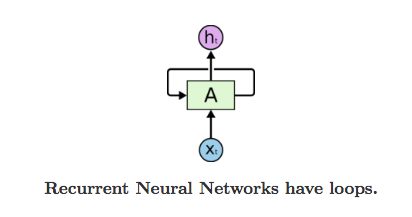
\includegraphics[width=\linewidth]{rnn.png}
	\caption{L'architettura base di una RNN}
	\label{fig:rnn}
\end{figure}
E' molto comune dare una rappresentazione \textit{unrolled} della rete per poterla ricondurre ad una rete neurale classica e comprenderne il funzionamento nel dettaglio.
\begin{figure}[H]
	\centering
	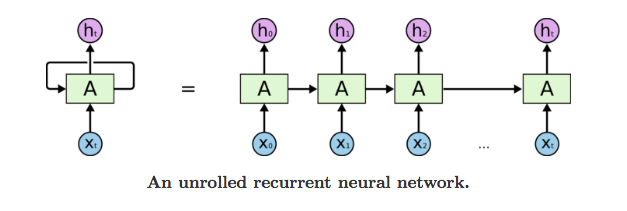
\includegraphics[width=\linewidth]{rnn_unrolled.png}
	\caption{La rappresentazione unrolled di una RNN}
	\label{fig:rnn_unrolled}
\end{figure}

Chiaramente, è possibile rendere più profonda una RNN, ed esistono diversi modi per farlo:
\begin{itemize}
	\item Aggiungere dei layer nascosti ricorrenti. Detta soluzione \textbf{stacked};
	\item Rendere il layer ricorrente una sotto-rete profonda;
	\item Aggiungere dei layer tra l'input e quello ricorrente;
	\item Aggiungere dei layer tra il ricorrente e l'output;
\end{itemize}

\subsection{LSTM}
Come evidenziato da Bengio et al.\cite{long_term}, il modello standard di RNN nella pratica soffre di un problema relativo alle \textbf{long-term dependencies}: man mano che la rete compie un alto numero di ripetizioni del layer ricorrente, le caratteristiche apprese dalla prime iterazioni iniziano a diventare meno rilevanti, quasi come se la rete iniziasse a dimenticare cosa ha fatto nel passato non recente. In molti casi è importante mantenere le informazioni che risalgono ad un passato meno recente.\\
\\
Per risolvere questo problema, Hochreiter et al.\cite{lstm} hanno presentato la più applicata implementazione di RNN, ovvero le reti \textbf{LSTM, Long Short Term Memory}.\\
Il layer ricorrente di una LSTM segue una precisa struttura, ed è chiamato \textbf{cella LSTM}. Mentre nelle RNN standard i layer ricorrenti sono composti da neuroni che applicano una qualsiasi funzione di attivazione, un layer LSTM è invece composto da quattro sotto-layer, che applicano delle funzioni più complesse.
\begin{figure}[H]
	\centering
	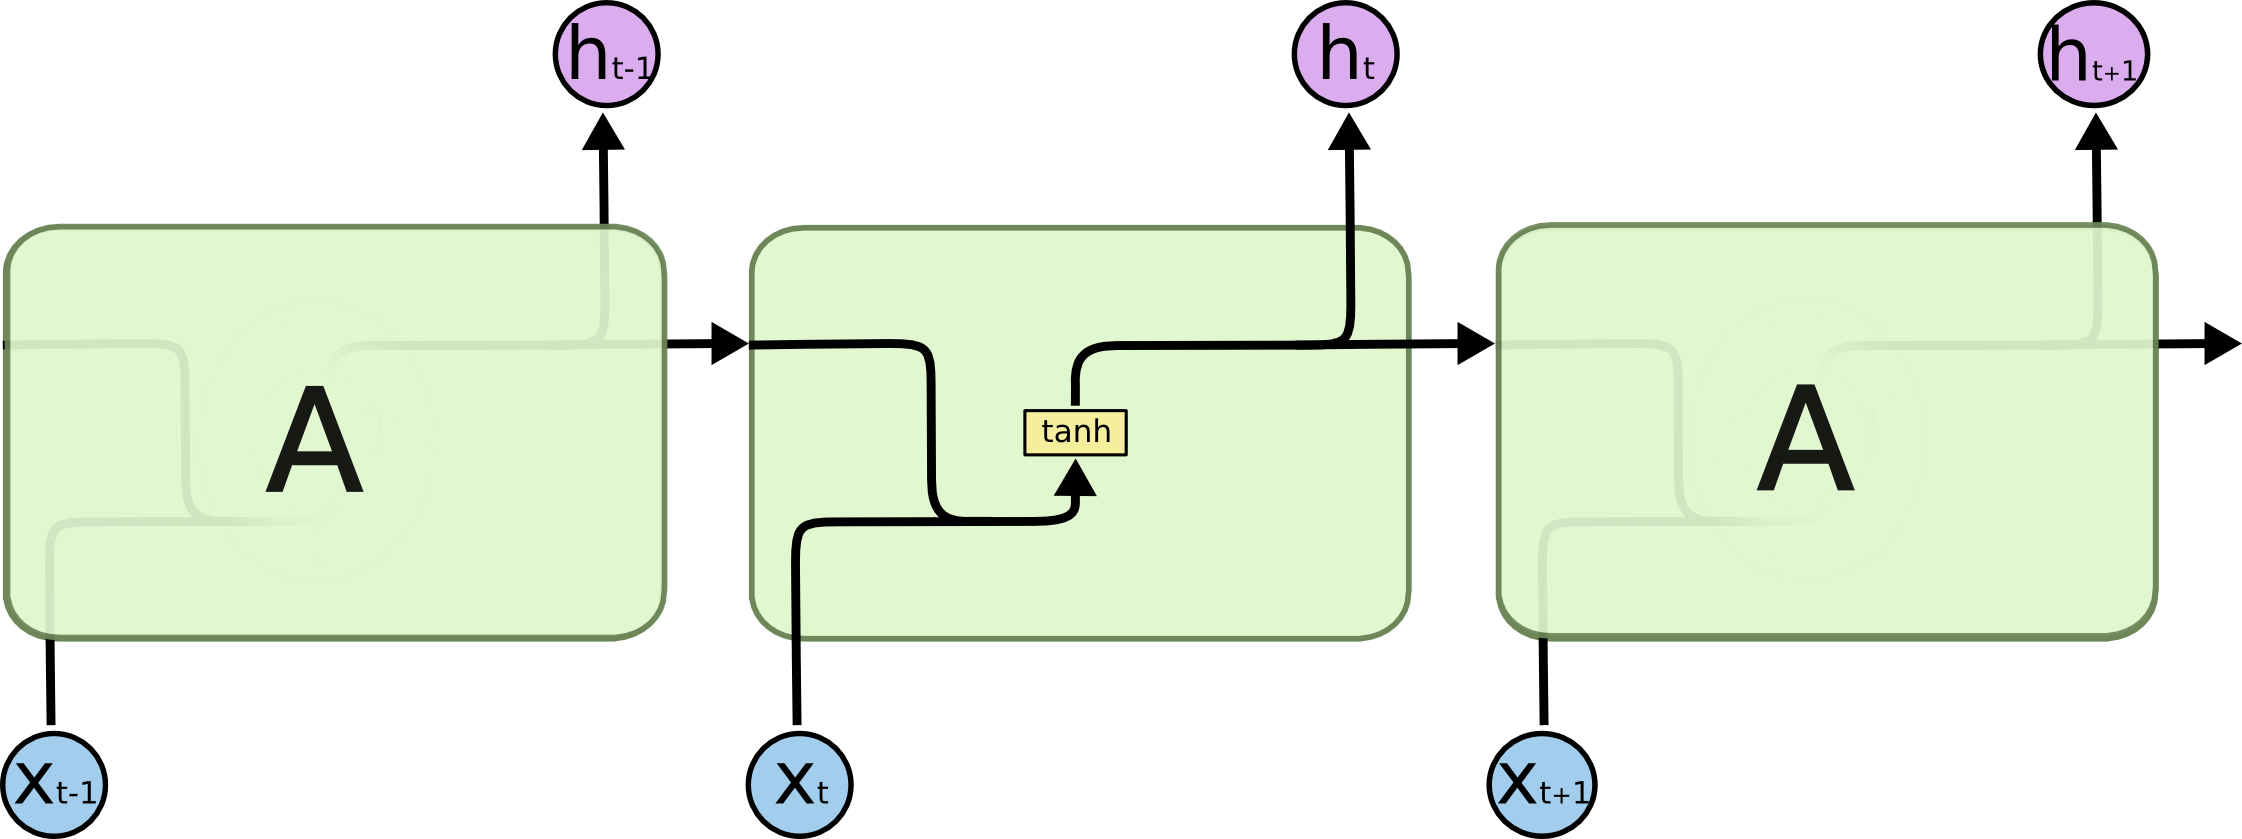
\includegraphics[width=\linewidth]{rnn_2.png}
	\caption{RNN unrolled standard. Nell'esempio viene usata la funzione di attivazione tangente iperbolica.}
	\label{fig:rnn_2}
\end{figure}
\begin{figure}[H]
	\centering
	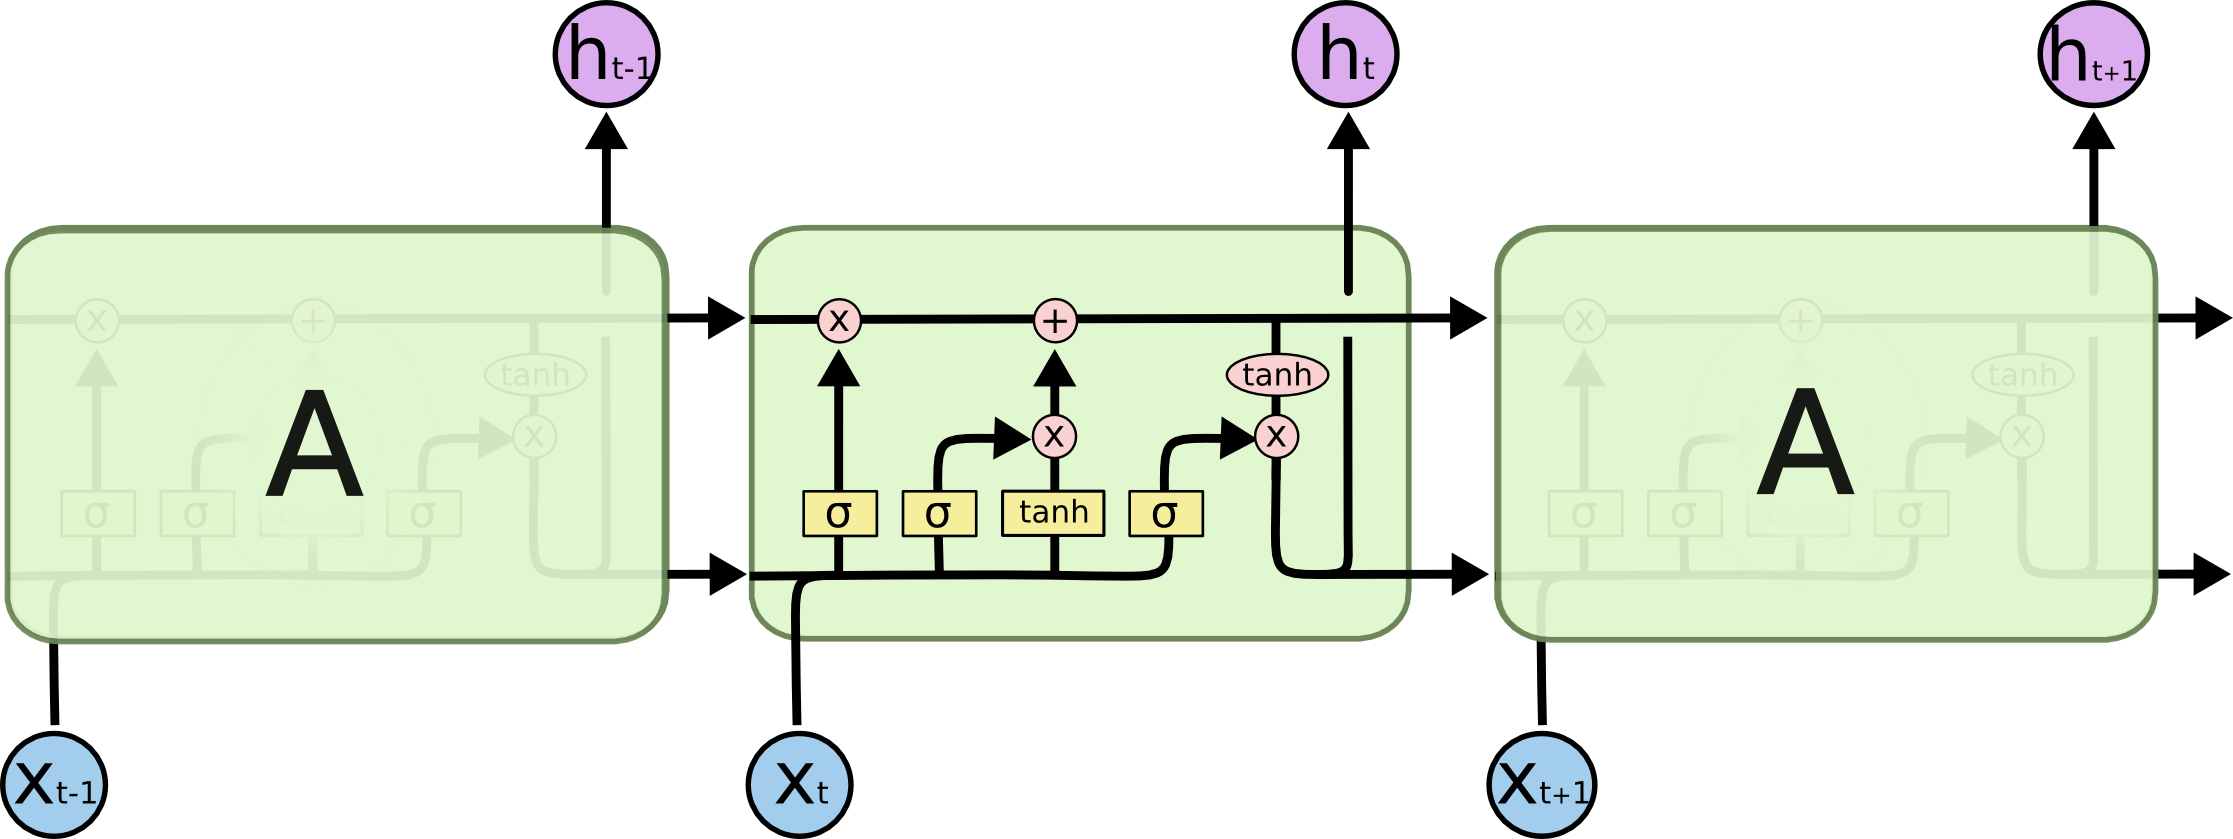
\includegraphics[width=\linewidth]{lstm.png}
	\caption{LSTM unrolled. I rettangoli gialli sono i quattro sotto-layer, di cui tre di essi applicano la semplice sigmoide, mentre l'altro la tangente iperbolica, mentre le figure rosa sono operazioni su vettori semplici.}
	\label{fig:lstm}
\end{figure}

La linea superiore della cella trasporta l'output superiore della cella precedente direttamente alla cella successiva, a meno di alcune operazioni lineari. Serve a mandare in avanti la conoscenza del passato senza modificarla troppo.\\
\\
La cella LSTM non segue necessariamente lo schema suddetto, ed esistono altre varianti, tutte accomunate dall'idea di avere un flusso che preservi le long-term dependencies.\\
La \textbf{hidden size}, cioè dimensione dell'hidden state, determina la dimensione dei quattro sotto-layer, ovvero il numero dei loro neuroni. Il numero totale dei neuroni presenti in una LSTM è allora dato dalla $hidden size * 4$. Tipicamente, \textbf{al crescere della hidden size cresce anche la capacità di memorizzazione della LSTM}.

\section{Autoencoder}
Un \textbf{autoencoder} è una tipologia di rete neurale che cerca di apprendere una rappresentazione "compressa" di un input, per poi tentare di ricostruirlo correttamente come output.\\
Nonostante questo possa sembrare confusionario ed inutile, una rete che impara una versione compressa dei dati si presta in maniera ottimale a risolvere una serie di task che altrimenti non avrebbero soluzioni adeguate. Sostanzialmente un autoencoder è un metodo per ottenere una rappresentazione di \textbf{dimensione ridotta} di un input di dimensionalità superiore.\\
\\
Un autoencoder prende i dati dall'input layer e li trasforma in una rappresentazione interna, detta \textbf{codifica} o \textbf{vettore latente}. Questa rappresentazione è ottima quando l'autoencoder con essa è in grado di ricostruire correttamente l'input, infatti il training di questa particolare rete consiste nel tentare di fornire un vettore latente ottimale per ciascun input.\\
Lo scopo finale non è quello di ricostruire perfettamente l'input (sarebbe abbastanza inutile) ma quello di estrarre dagli input \textbf{questo vettore latente ottimale che conterrà le loro principali caratteristiche}. In altre parole, si pone di estrarre feature rilevanti dall'input.\\
La compressione e la decompressione vengono effettuate attraverso delle funzioni che imparano automaticamente, senza l'ausilio dell'uomo (\textbf{unsupervised}), dai sample di un training set. In quasi tutti i contesti in cui sono usati gli autoencoder, le funzioni di compressione e decompressione sono implementare con reti neurali (nel nostro caso \textbf{LSTM}).\\
\\
Per compiere la ricostruzione è necessario che input e output layer siano della stessa dimensione, tuttavia, al fine di permettere alla rete di estrarre le feature dagli input, il layer nascosto che genera la codifica, detto \textbf{coding layer}, dovrà necessariamente essere di dimensione minore degli input e output layer. Si parla di autoencoder \textbf{undercomplete}.\\
\\
Come detto un autoencoder è sempre composto da:
\begin{itemize}
	\item Un \textbf{encoder}, solitamente una rete neurale che riduce l'input nella codifica. Anche detta \textit{rete ricognitiva};
	\item Un \textbf{decoder}, solitamente una rete neurale che ricostruisce l'input dell'encoder a partire dalla codifica. Anche detta \textit{rete generativa};
\end{itemize}
Encoder e decoder sono simmetrici rispetto al coding layer.
\begin{figure}[H]
	\centering
	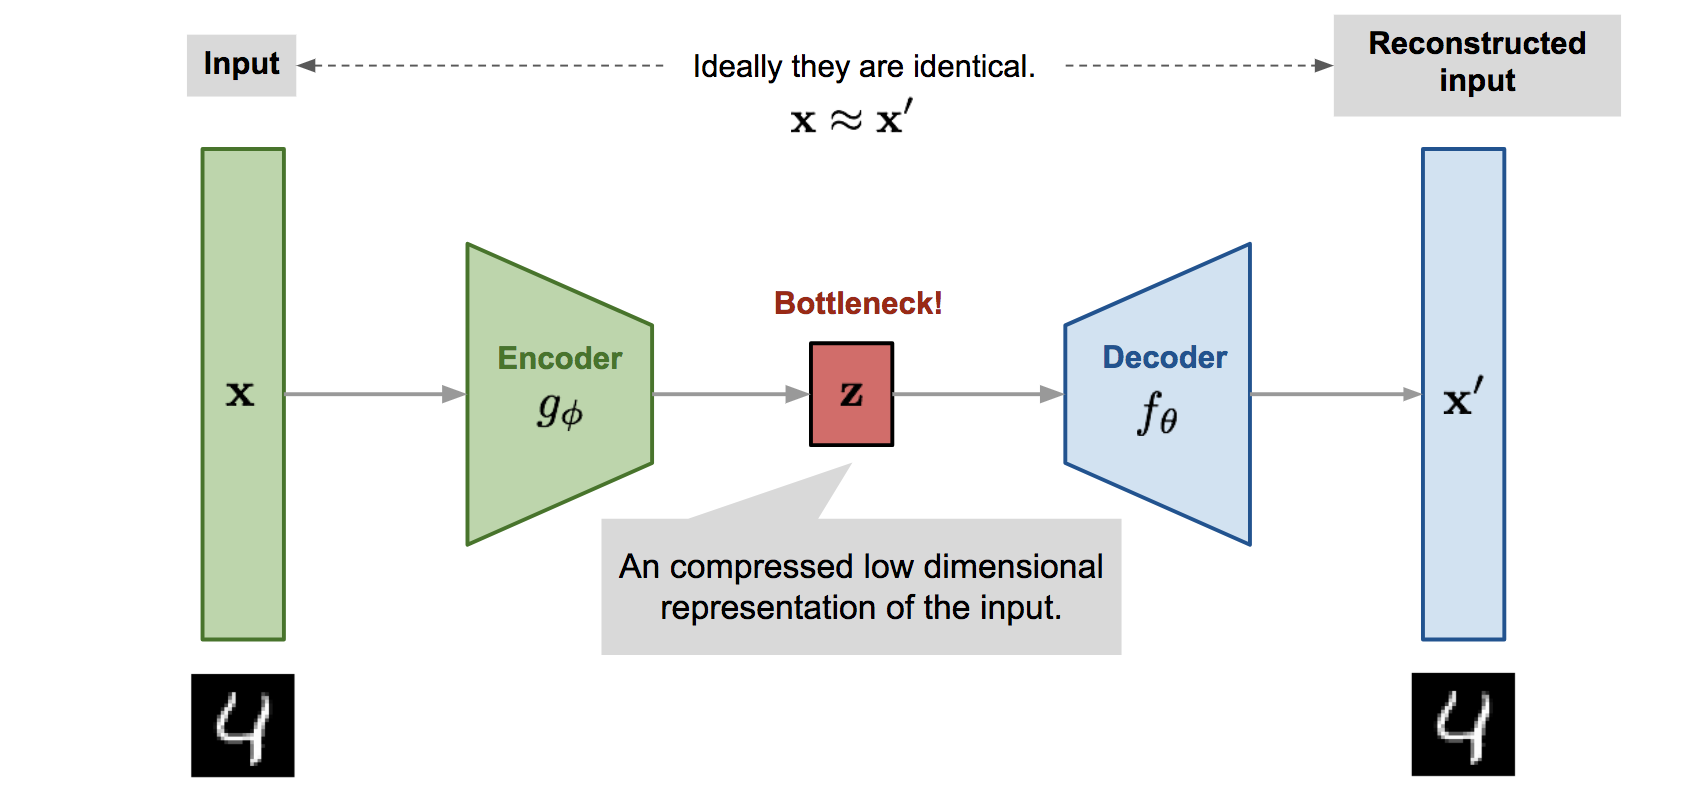
\includegraphics[width=\linewidth]{autoencoder.png}
	\caption{Schema di un autoencoder.}
	\label{fig:autoencoder}
\end{figure}

Gli autoencoder sono usati principalmente per fare \textbf{dimensionality reduction}, dato che la codifica è una rappresentazione ridotta di ogni input, ma anche \textbf{generazione di sample}, ovvero generare nuovi dati a partire da codifiche arbitrarie.\\
\\
Come una qualsiasi altra rete neurale, gli autoencoder possono essere resi più profondi aggiungendo layer nascosti, sia dal lato dell'encoder che dal lato del decoder. In tal caso si parla di \textbf{autoencoder stacked}.\\
In generale, un maggior livello di profondità permette alla rete di comprendere pattern più complessi, tuttavia una profondità troppo alta rende il rischio di overfitting più alto.

\subsection{Variational Autoencoders}
Come i tradizionali autoencoder, i \textbf{Variational Autoencoders} (VAEs) cercano di ricostruire gli input utilizzando un encoder e un decoder. Anche in questo caso, l'output dell'encoder è una rappresentazione compressa dell'input, e il decoder impara a ricostruire l'input iniziale prendendo come punto di partenza la rappresentazione compressa generata dall'encoder.\\
Ciò che rende particolare questa tipologia di autoencoder è che il modello prevede un \textbf{approccio probabilistico} per descrivere le osservazioni nello spazio latente.\\
Anziché costruire un autoencoder il cui output è un singolo valore per ogni attributo del vettore dei fattori latenti, questo viene formulato in maniera tale da descrivere una \textbf{distribuzione di probabilità} per ogni attributo latente, tipicamente una distribuzione normale.\\
Costruendo l'encoder in questo modo otteniamo un range di possibili valori (la distribuzione, appunto), e l'esito è quello di forzare il modello a rappresentare l'input in uno spazio latente continuo e regolare rispetto ai valori iniziali. Per ogni campione della \textbf{distribuzione latente} ci aspettiamo che il decoder sia in grado di ricostruire l'input. I valori che sono vicini uno all'altro nello spazio latente in questo modo vengono ricostruiti in maniera simile. 

\section{Modello proposto}
\subsection{Architettura e motivazione}
Il modello proposto è composto da quattro componenti fondamentali:
\begin{itemize}
	\item Il primo componente è l'\textbf{encoder} costituito da una rete \textbf{Stacked LSTM}. Questa prende in input un vettore che descrive una TS;
	\item Successivamente, vi è una componente adibita al mappare l'\textbf{hidden vector} ottenuto dall'encoder in un vettore dei \textbf{fattori latenti}. In questo layer viene effettuato il train dei punti nello spazio latente per avere media nulla e varianza unitaria (il perché è discusso nella prossima sezione relativa al training);
	\item La componente successiva deve fare il processo inverso al precedente, cioè mappare il vettore latente nel vettore input per il decoder;
	\item l'ultima componente è il \textbf{decoder} che è una rete Stacked LSTM speculare a quella dell'encoder che prende il singolo vettore ricevuto e lo mappa in una sequenza di vettori in output, cioè cerca di ricostruire gli input.
\end{itemize}

L'idea dietro il modello è quella che, attraverso le LSTM, si possano ottenere le feature più significative delle serie temporali in input.\\
Se il modello converge vuol dire che il vettore latente è sufficientemente preciso nel ricostruire l'input iniziale. Il vettore latente che si ottiene viene poi utilizzato per effettuare il clustering con k-means.\\
\\
Il cuore del modello è sicuramente nel'utilizzo delle LSTM: nello studio delle serie temporali, le LSTM sono attualmente considerate il miglior "strumento" per ottenere buoni risultati nella maggior parte dei casi. Il problema delle serie temporali è infatti quello di avere molto rumore e di nascondere influenze nascoste nei dati.\\
Modelli troppo semplici non si comportano adeguatamente su questo tipo di dati, mentre le LSTM riescono a superare questi problemi, ma anche quelli relativi agli andamenti irregolari, come ad esempio l'avere linearità e non linearità nella stessa serie temporale.

\subsection{Training e iperparametri}
L'obiettivo del training è quello di imparare la funzione di identità in maniera tale che la sequenza dei vettori di input e output sia simile.\\ 
Come detto, è stato usato un approccio probabilistico: l'obiettivo è ricavare i parametri della distribuzione normale dell'hidden vector, cioè $\mu$ e $\sigma$, cercando di minimizzare il \textbf{logaritmo di verosimiglianza} dell'input sotto questa distribuzione.\\
La scelta di imporre la distribuzione normale è stata dettata sia dalla letteratura disponibile, che consiglia questa distribuzione, ma anche del fatto che altrimenti non sarebbe stato possibile utilizzare la tecnica della discesa stocastica del gradiente nella variante \textbf{Adam} (ADAptive Moment estimation), anch'esso in letteratura ritenuto il miglior optimizer per questo tipo di problemi.
\\
Durante il training è stato necessario lavorare sui tanti \textbf{iperparametri} della rete. I principali, sui quali si è data maggiore attenzione, sono:
\begin{itemize}
	\item \textbf{Number of layers}, indicante il numero di LSTM messe in stack. E' stato scelto 2 per tutti i dataset, per evitare di dare troppa complessità al modello;
	
	\item \textbf{Hidden size}, indicante la dimensione dell'hidden state, e quindi della singola cella LSTM. E' stato scelto \textbf{un valore dipendente dalla tipologia di time series: valori minori se esse avevano andamenti tendenzialmente lineari, altrimenti maggiori.}, così da avere migliori capacità di memorizzazione;
	
	\item \textbf{Vector size}, indicante la dimensione dei vettori latenti. E' stato scelto \textbf{un valore proporzionato alla lunghezza delle time series dei diversi dataset}, così da avere buone capacità di compressione;
	
	\item \textbf{Learning rate}, indicante il tasso di funzionamento del Gradient Descent. E' stato scelto \textbf{osservando come si comportava la funzione di loss durante il training, diminuendolo in caso di reti molto rapide nella convergenza oppure con grandi fluttuazioni della loss};
	
	\item \textbf{Max iterations}, indicante il numero massimo di sessioni di training, ovvero il numero di applicazioni del Gradient Descent per correggere i pesi della rete. E' stato scelto \textbf{osservando come si comportava la funzione di loss durante il training, aumentandole in caso di reti con difficoltà nella convergenza};
	
\end{itemize}
Tutti gli iperaparametri sono riportati nel notebook relativo all'autoencoder. Ciascun dataset ha il suo setting più opportuno. Il setting non è stato immediato e si è ricorso alla \textbf{random search} per poter trovarne una buona combinazione.\\

\section{Clustering con k-Means}
Per poter sfruttare la riduzione della dimensionalità compiuta dall'autoencoder, tutto il test set (di default corrispondente al 20\% del dataset) viene dato in input all'autoencoder per estrarne i relativi vettori latenti, ovvero la codifica delle TS di test.\\
Il k-Means viene lanciato cinque volte, seguendo questa regola. Sia n il numero di classi di un dataset:
\begin{enumerate}[(i)]
	\item Se $n\leq3$, allora si esegue da $2-$Means a $6-$Means;
	\item Se $n>2$, allora si esegue da $n-2-$Means ad $n+2-$Means.
\end{enumerate}
L'implementazione utilizzata è quella di Scikit-Learn, la quale viene retirata 100 volte (tramite il parametro $n\_init$), in modo tale che venga scelto il clustering migliore su 100 tentativi. Non viene fornito nessun random state in input.\\
Il k-Means usa come funzione di distanza quella euclidea, che risulta accettabile poiché i vettori latenti non sono delle TS, quindi la distanza DTW non è pienamente adatta, oltre che dispendiosa in termini di computazione.\\
\\
Per ciascuna esecuzione di k-Means viene mostrato il plot del clustering sui sample di test. Le metriche di valutazione, sia interne che esterne, sono tutte accumulate in un DataFrame di Pandas, esportato successivamente in CSV.

\subsection{Valutazione dei risultati}
Per alcuni dataset, come ECG5000, ECG200, TwoLeadECG, PhalangesOutlineCorrect, ChlorineConcentration, questa ricerca ha portato miglioramenti in tutti gli score, mentre per gli altri dataset la ricerca non comportava alcun cambiamento sostanziale.
Di seguito sono riportati i risultati del clustering effettuato sui vari dataset in esame, con i valori migliori per gli iperapametri.

\subsubsection{ECG5000}
\begin{center}
	\pgfplotstabletypeset[
	col sep=comma,
	string type,
	every head row/.style={
		before row={\hline
			\multicolumn{1}{c|}{\textbf{ECG5000}} &
			\multicolumn{2}{c|}{Internal} & \multicolumn{4}{c}{External} \\
		},
		after row=\hline
	},
	every last row/.style={after row=\hline},
	]{metrics/autoencoder/ECG5000_metrics.csv}
	\begin{table}[H]
		\centering
		\caption{k-Means sui vettori latenti del test set di ECG5000.}
	\end{table}
\end{center}

\subsubsection{ECG200}
\begin{center}
	\pgfplotstabletypeset[
	col sep=comma,
	string type,
	every head row/.style={
		before row={\hline
			\multicolumn{1}{c|}{\textbf{ECG200}} &
			\multicolumn{2}{c|}{Internal} & \multicolumn{4}{c}{External} \\
		},
		after row=\hline
	},
	every last row/.style={after row=\hline},
	]{metrics/autoencoder/ECG200_metrics.csv}
	\begin{table}[H]
		\centering
		\caption{k-Means sui vettori latenti del test set di ECG200.}
	\end{table}
\end{center}

\subsubsection{ChlorineConcentration}
\begin{center}
	\pgfplotstabletypeset[
	col sep=comma,
	string type,
	every head row/.style={
		before row={\hline
			\multicolumn{1}{c|}{\textbf{Chlorine}} &
			\multicolumn{2}{c|}{Internal} & \multicolumn{4}{c}{External} \\
		},
		after row=\hline
	},
	every last row/.style={after row=\hline},
	]{metrics/autoencoder/ChlorineConcentration_metrics.csv}
	\begin{table}[H]
		\centering
		\caption{k-Means sui vettori latenti del test set di ChlorineConcentration.}
	\end{table}
\end{center}

\subsubsection{FordA}
\begin{center}
	\pgfplotstabletypeset[
	col sep=comma,
	string type,
	every head row/.style={
		before row={\hline
			\multicolumn{1}{c|}{\textbf{FordA}} &
			\multicolumn{2}{c|}{Internal} & \multicolumn{4}{c}{External} \\
		},
		after row=\hline
	},
	every last row/.style={after row=\hline},
	]{metrics/autoencoder/FordA_metrics.csv}
	\begin{table}[H]
		\centering
		\caption{k-Means sui vettori latenti del test set di FordA.}
	\end{table}
\end{center}

\subsubsection{FordB}
\begin{center}
	\pgfplotstabletypeset[
	col sep=comma,
	string type,
	every head row/.style={
		before row={\hline
			\multicolumn{1}{c|}{\textbf{FordB}} &
			\multicolumn{2}{c|}{Internal} & \multicolumn{4}{c}{External} \\
		},
		after row=\hline
	},
	every last row/.style={after row=\hline},
	]{metrics/autoencoder/FordB_metrics.csv}
	\begin{table}[H]
		\centering
		\caption{k-Means sui vettori latenti del test set di FordB.}
	\end{table}
\end{center}

\subsubsection{PhalangesOutlinesCorrect}
\begin{center}
	\pgfplotstabletypeset[
	col sep=comma,
	string type,
	every head row/.style={
		before row={\hline
			\multicolumn{1}{c|}{\textbf{Phalanges}} &
			\multicolumn{2}{c|}{Internal} & \multicolumn{4}{c}{External} \\
		},
		after row=\hline
	},
	every last row/.style={after row=\hline},
	]{metrics/autoencoder/PhalangesOutlinesCorrect_metrics.csv}
	\begin{table}[H]
		\centering
		\caption{k-Means sui vettori latenti del test set di PhalangesOutlinesCorrect.}
	\end{table}
\end{center}

\subsubsection{RefrigerationDevices}
\begin{center}
	\pgfplotstabletypeset[
	col sep=comma,
	string type,
	every head row/.style={
		before row={\hline
			\multicolumn{1}{c|}{\textbf{Refrigeration}} &
			\multicolumn{2}{c|}{Internal} & \multicolumn{4}{c}{External} \\
		},
		after row=\hline
	},
	every last row/.style={after row=\hline},
	]{metrics/autoencoder/RefrigerationDevices_metrics.csv}
	\begin{table}[H]
		\centering
		\caption{k-Means sui vettori latenti del test set di RefrigerationDevices.}
	\end{table}
\end{center}

\subsubsection{TwoLeadECG}
\begin{center}
	\pgfplotstabletypeset[
	col sep=comma,
	string type,
	every head row/.style={
		before row={\hline
			\multicolumn{1}{c|}{\textbf{TwoLeadECG}} &
			\multicolumn{2}{c|}{Internal} & \multicolumn{4}{c}{External} \\
		},
		after row=\hline
	},
	every last row/.style={after row=\hline},
	]{metrics/autoencoder/TwoLeadECG_metrics.csv}
	\begin{table}[H]
		\centering
		\caption{k-Means sui vettori latenti del test set di TwoLeadECG.}
	\end{table}
\end{center}

\subsubsection{TwoPatterns}
\begin{center}
	\pgfplotstabletypeset[
	col sep=comma,
	string type,
	every head row/.style={
		before row={\hline
			\multicolumn{1}{c|}{\textbf{TwoPatterns}} &
			\multicolumn{2}{c|}{Internal} & \multicolumn{4}{c}{External} \\
		},
		after row=\hline
	},
	every last row/.style={after row=\hline},
	]{metrics/autoencoder/TwoPatterns_metrics.csv}
	\begin{table}[H]
		\centering
		\caption{k-Means sui vettori latenti del test set di TwoPatterns.}
	\end{table}
\end{center}

Da questi risultati è possibile fare una serie di osservazioni sulle misure:
\begin{enumerate}
	\item Le \textbf{misure interne sono molto influenzate dal numero di cluster}, andando a peggiorare man mano che il numero cresce.\\
	Questo, chiaramente, dipende molto dalla disposizione dei dati nello spazio e anche dal tipo di algoritmo di clustering: k-Means, infatti, non ottimizza la densità dei cluster, a differenza di altri come DBSCAN;
	\item Le \textbf{misure esterne sono molto suscettibili con piccoli dataset}, infatti, nel caso di ECG200, si hanno ARI ed FMI abbastanza bassi.\\
	Il motivo risiede nel fatto che le metriche esterne sono basate su conteggi non pesati;
	\item Le misure di \textbf{purity e relative purity sono abbastanza indipendenti dal numero di cluster}.\\
	Questo potrebbe significare che sono più influenzare dalla natura del dataset e dalle caratteristiche che l'autoencoder è stato in grado di estrarre, piuttosto che dal numero di cluster.
\end{enumerate}

Inoltre, è stato possibile fare le seguenti osservazioni sul modello e sui dataset:
\begin{enumerate}	
	\item Nei \textbf{dataset degli elettrocardiogrammi le misure esterne sono tendenzialmente alte}. Questo significa che l'autoencoder è riuscito a estrarre quelle caratteristiche che gli autori dei dataset hanno usato per fare il labelling degli elettrocardiogrammi.\\
	Questo non accade per gli altri dataset, o almeno non con gli stessi score;
	\item \textbf{Le caratteristiche delle TS molto "rumorose"}\footnote{hanno dei pattern che continuamente alternano valori alti e valori bassi} \textbf{non riescono ad essere estratte bene dall'autoencoder}, e questo si rispecchia nelle misure interne basse e nelle misure esterne che ricordano quelle del random labelling. Questo accade per FordA, FordB, RefrigerationDevices e TwoPatterns;
\end{enumerate}

\chapter{Analisi comparativa} \label{chap:comparison}
\section{DTW: Dynamic Time Warping}
Il \textbf{Dynamic Time Warping} (DTW)\cite{dtw}è un algoritmo per misurare la similarità tra due TS, calcolandone il match ottimale.\\
\\
A differenza delle classiche funzioni di distanza, come quella Euclidea o la Manhattan, essa effettua un confronto di tipo \textbf{elastico} (non-lineare) tra i punti delle due TS a confronto: Esse non sono confrontate 1-a-1, matchando l'$i$-esimo punto della TS A con l'$i$-esimo punto della TS B, bensì 1-a-n, matchando un punto della TS A con uno o più punti della TS B.\\
Il confronto tra due punti matchati avviene sempre con una metrica classica, come quella Euclidea. Tutte le singole distanze tra i punti sono conservate in una \textbf{matrice di distanza}.\\
\\
Siano A e B due TS a confronto, vengono imposti i seguenti vincoli nel clacolo del DTW:
\begin{itemize}
	\item Un punto di una TS può essere matchato con uno o più punti dell'altra TS;
	\item Il match tra due punti può avviene se e solo se le due TS hanno la stessa monotonia nei rispettivi punti;
	\item Il primo punto della TS A è matchato con il primo della TS B;
	\item L'ultimo punto della TS A è matchato con l'ultimo della TS B; 
\end{itemize}
\begin{figure}[H]
	\centering
	\begin{subfigure}{.5\textwidth}
		\centering
		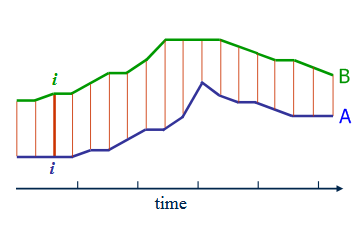
\includegraphics[width=.9\linewidth]{euclidean.png}
		\caption{Distanza Euclidea (lineare)}
		\label{fig:distance_euclidean}
	\end{subfigure}%
	\begin{subfigure}{.5\textwidth}
		\centering
		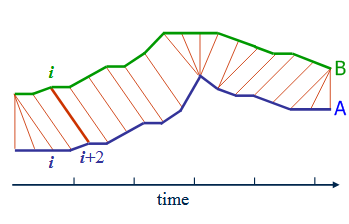
\includegraphics[width=.9\linewidth]{dtw.png}
		\caption{DTW (elastica)}
		\label{fig:distance_dtw}
	\end{subfigure}
	\caption{Confronto tra distanza Euclidea e DTW}
	\label{fig:distance}
\end{figure}
In altre parole, il DTW cerca di "allineare" al meglio le due TS, facendo in modo che entrambe proseguano con lo stesso andamento.\\
\\
La similarità del DTW produce buoni risultati per le TS che rappresentano uno stesso evento ma che sono di lunghezza differente, ad esempio quando entra in gioco uno sfasamento temporale.\\
Un individuo che pronuncia una stessa frase con lo stesso tono ma con velocità differente produrrebbe due TS molto differenti. Se esse venissero confrontate linearmente, non si potrebbe riconoscere che, difatti, l'individuo che ha prodotto tali frequenze è lo stesso. Con un confronto tramite DTW ciò viene ovviato.\\
\\
L'algoritmo compie una ricerca nella matrice di distanza, di spazio $O(mn)$, dove $m$ ed $n$ sono le lunghezze delle due TS confrontate.
Dunque, al caso pessimo e con TS molto grandi (es. centinaia di punti), il calcolo del DTW richiede un tempo impraticabile. In letteratura, perciò, sono state definite alcune implementazioni veloci, come \textit{PrunedDTW}, \textit{SparseDTW} e \textit{FastDTW}, che tentano di accelerarne il calcolo. Ciò nonostante, la tecnica resta complessa in termini di tempo e di spazio, sopratutto in caso di dataset ad alta dimensionalità.\\

\section{Confronto con k-Means di TSLearn}
Il clustering mediante l'impiego di DWT è stato realizzato sfruttando la libreria TSLearn.
Essa, infatti, come evidenziato dal nome stesso, consiste in una specializzazione del Machine Learning focalizzato sulle Time Series.
La libreria non solo offre metodi per il calcolo delle metriche proprie delle TS (\textit{DTW},\textit{Soft-DTW}, ecc.), ma anche veri e propri algoritmi di Machine Learning in una variante modificata \textit{ad hoc} per le TS, sia di tipo supervised che unsupervised (es. \textit{SVM}, \textit{TimeSeriesKMeans}).\\
\\
Proprio uno di questi algoritmi, \textit{TimeSeriesKMeans}, è stato impiegato per il nostro esperimento.
Esso consiste in una versione modificata del noto algoritmo di clustering, abile nel calcolo dei cluster usando non solo la metrica euclidea, ma anche il DTW e il Soft-DTW.\\
\\
Di seguito sono riportati i risultati del clustering dei dataset in esame, con però alcune premesse:
\begin{itemize}
	\item Il Silhouette Coefficient non è presente in alcun dataset, data l'impraticabilità di calcolo su dataset di grandi dimenioni;
	\item Non viene riportata la Relative Purity perché introdotta successivamente al calcolo di questi risultati, e una sua introduzione avrebbe richiesto un computo troppo oneroso;
	\item Per avere un riscontro diretto con le labels presente nei dataset, il numero di cluster calcolati corrisponde al numero di classi presenti nel dataset;
\end{itemize}

\begin{center}
	\pgfplotstabletypeset[
	col sep=comma,
	string type,
	every head row/.style={
		before row={\hline
			\multicolumn{3}{c|}{\textbf{}} &
			\multicolumn{1}{c|}{Internal} & \multicolumn{3}{c}{External} \\
		},
		after row=\hline
	},
	every last row/.style={after row=\hline},
	]{metrics/dtw/All_dtw.csv}
	\begin{table}[H]
		\centering
		\caption{k-Means con DTW sui dataset in esame con relative misure.}
	\end{table}
\end{center}

Da questi risultati è possibile fare una serie di osservazioni:
\begin{enumerate}
	\item In \textit{ECG5000}, \textbf{l'autoencoder e TSLearn con 5-Means hanno tutti gli score molto simili}.\\
	L'autoencoder è riuscito ad estrarre bene le caratteristiche degli elettrocardiogrammi, come intuito dall'analisi precedente;

	\item In \textit{ECG200}, \textbf{l'autoencoder con 2-Means ha tutti gli score leggermente migliori rispetto a TSLearn}.\\
	Le motivazioni sono le stesse di ECG5000;

	\item In \textit{ChlorineConcentration}, \textbf{l'autoencoder e TSLearn su 3-Means hanno tutti gli score molto simili}, se non per una leggera differenza per FMI.\\
	L'autoencoder è riuscito ad estrarre bene le caratteristiche di questo tipo di TS, cosa non intuita dall'analisi precedente;

	\item In \textit{FordA}, \textbf{l'autoencoder con 2-Means ha tutti gli score ben peggiori rispetto a TSLearn}, ad eccezione del FMI, dove in entrambi i casi è comunque non ottimale.\\ L'autoencoder non è riuscito ad estrarre bene le caratteristiche di queste TS "rumorose", come intuito dall'analisi precedente;

	\item In \textit{FordB}, \textbf{l'autoencoder con 2-Means ha il DB ben peggiore di quelli di TSLearn}, mentre gli score esterni risultano simili.\\
	Similmente a FordA, l'autoencoder non è riuscito ad estrarre bene le caratteristiche di queste TS, come intuito dall'analisi precedente;

	\item In \textit{PhalangesOutlineCorrect}, \textbf{l'autoencoder con 2-Means ha qualche score leggermente peggiore rispetto a TSLearn}.\\
	L'autoencoder è riuscito ad estrarre abbastanza bene le caratteristiche di questo tipo di TS, magari c'è bisogno di alcune modifiche agli iperparametri per poter migliorarne la qualità;

	\item In \textit{RefrigerationDevices}, \textbf{l'autoencoder con 3-Means ha tutti gli score ben peggiori rispetto a TSLearn}, ad eccezione del FMI, dove in entrambi i casi è comunque non ottimale.\\
	Quasi identicamente a FordA, l'autoencoder non è riuscito ad estrarre bene le caratteristiche di queste TS "rumorose", come intuito dall'analisi precedente;

	\item In \textit{TwoLeadECG}, \textbf{l'autoencoder e TSLearn con 2-Means hanno tutti gli score molto simili}, ad eccezione del DB dove l'autoencodere è migliore.\\
	Questa analisi non è pienamente affidabile perché il test set fornito è troppo piccolo, quindi gli score sono soggetti a molte variazioni in caso di riesecuzioni.

	\item In \textit{TwoPatterns}, \textbf{l'autoencoder con 4-Means ha tutti gli score ben peggiori rispetto a TSLearn}, ad eccezione del DB, dove resta comunque non ottimale.\\
	Similmente a FordA, l'autoencoder non è riuscito ad estrarre bene le caratteristiche di queste TS "rumorose", come intuito dall'analisi precedente;
\end{enumerate}

\section{Confronto con altre tecniche di feature extraction and selection}
Sono stati reperiti alcuni risultati di clustering sui dataset in esame attuando però altre tecniche di feature extraction and selection. Il clustering è stato fatto con k-Means con k pari al numero di classi del dataset e su un numero differente di feature estratte in modo diverso:
\begin{itemize}
	\item \textbf{Tutte le feature estratte} da \textit{TSFresh};
	\item \textbf{Feature rilevanti} selezionate da \textit{TSFresh};
	\item Feature rilevanti selezionate dall'algoritmo \textbf{NDFS};
	\item Feature rilevanti selezionate dall'algoritmo \textbf{Lap Score}.
\end{itemize}
I seguenti risultati riportano solo gli score silhouette, Davies-Bouldin e purity, quindi verranno usati solamente questi per il confronto.

\subsubsection{ECG5000}
\begin{figure}[H]
	\centering
	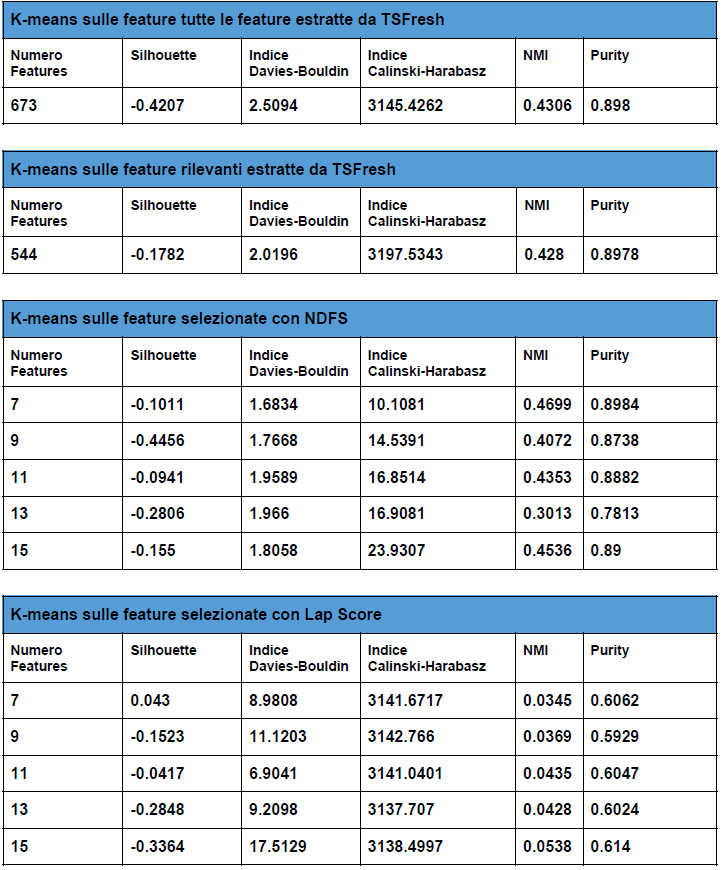
\includegraphics[width=0.9\linewidth]{av/ecg5000_av.png}
	\caption{ECG5000 con tecniche di feature extraction and selection.\\
	\\
	\textbf{L'autoencoder ha migliore silhouette rispetto a tutti gli algoritmi}. DB e Purity sono simili per autoencoder, TSFresh ed NDFS. Lap Score ha gli score peggiori.}
	\label{fig:ecg5000_av}
\end{figure}

\subsubsection{ECG200}
\begin{figure}[H]
	\centering
	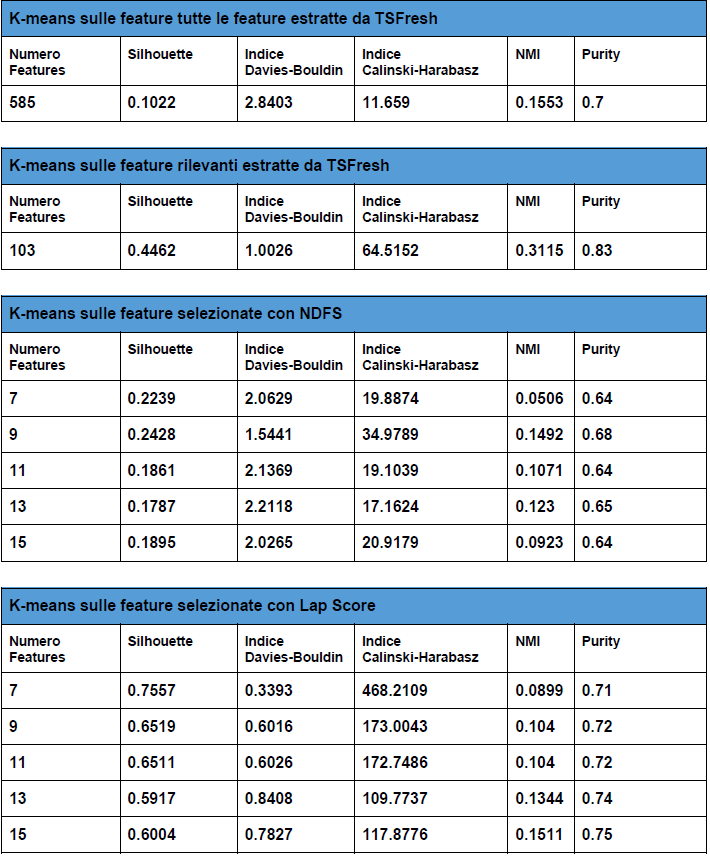
\includegraphics[width=0.9\linewidth]{av/ecg200_av.png}
	\caption{ECG200 con tecniche di feature extraction and selection.\\
	\\
	\textbf{L'autoencoder ha migliore DB rispetto a tutti gli algoritmi, e silhouette migliore rispetto a TSFresh e NDFS, ma peggiore rispetto a Lap Score}. La purity è simile per autoencoder, TSFresh e Lap Score.}
	\label{fig:ecg200_av}
\end{figure}

\subsubsection{ChlorineConcentration}
\begin{figure}[H]
	\centering
	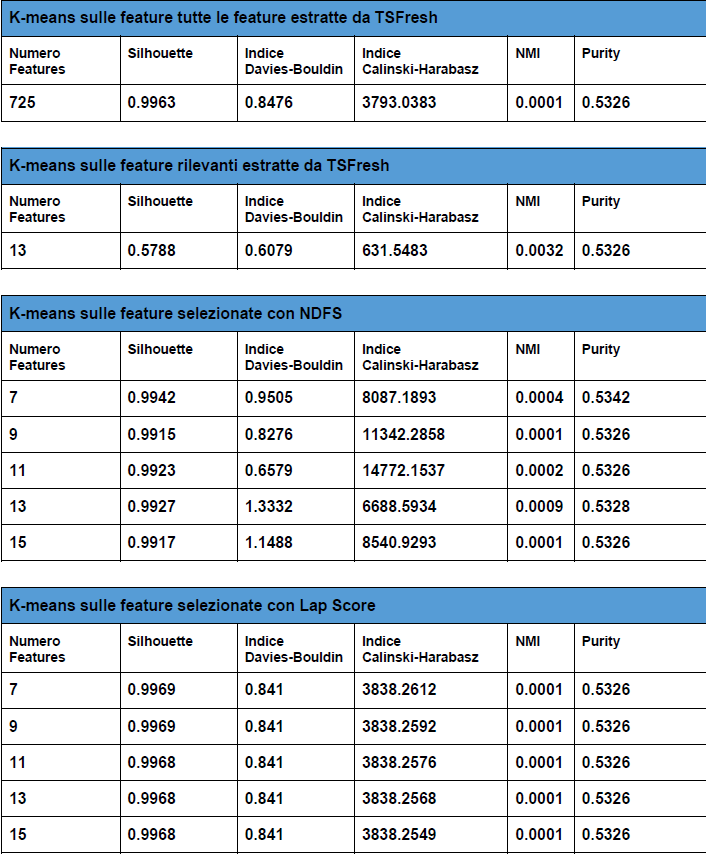
\includegraphics[width=0.9\linewidth]{av/chlorine_av.png}
	\caption{ChlorineConcentration con tecniche di feature extraction and selection.\\
	\\
	\textbf{L'autoencoder ha purity simile a tutti e quattro gli algoritmi}, DB peggiore solo rispetto a TSFresh per feature rilevanti, e silhouette peggiore in tutti i casi, specialmente rispetto ad NDFS e Lap Score, nei quali è quasi massima.}
	\label{fig:chlorine_av}
\end{figure}

\subsubsection{FordA}
\begin{figure}[H]
	\centering
	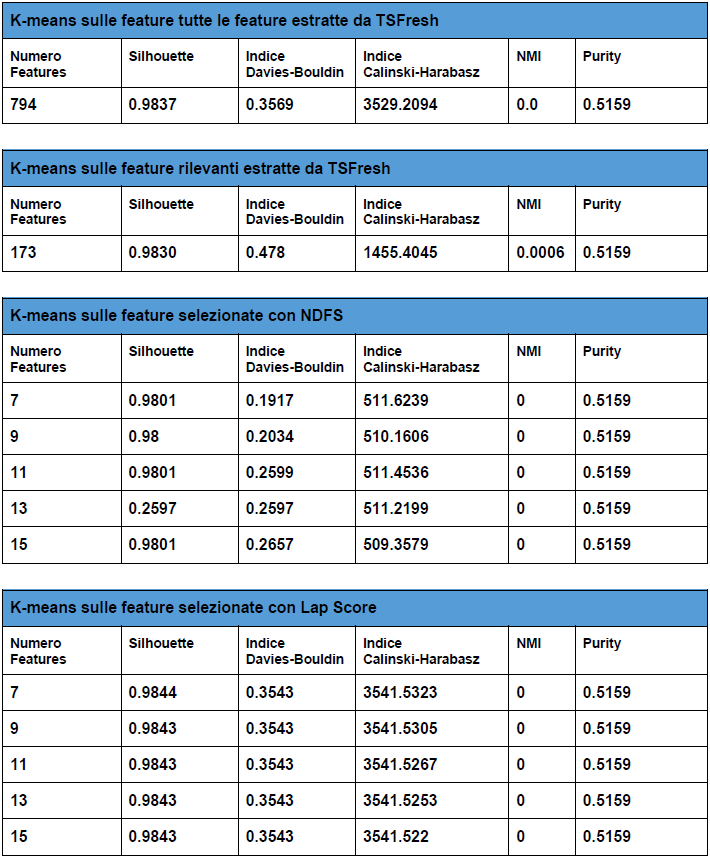
\includegraphics[width=0.9\linewidth]{av/forda_av.png}
	\caption{FordA con tecniche di feature extraction and selection.\\
	\\
	\textbf{L'autoencoder ha silhouette e DB di gran lunga peggiori rispetto a quattro gli algoritmi}, mentre la purity è simile in tutti i casi. DB è quasi ottimale con NDFS.}
	\label{fig:forda_av}
\end{figure}

\subsubsection{FordB}
\begin{figure}[H]
	\centering
	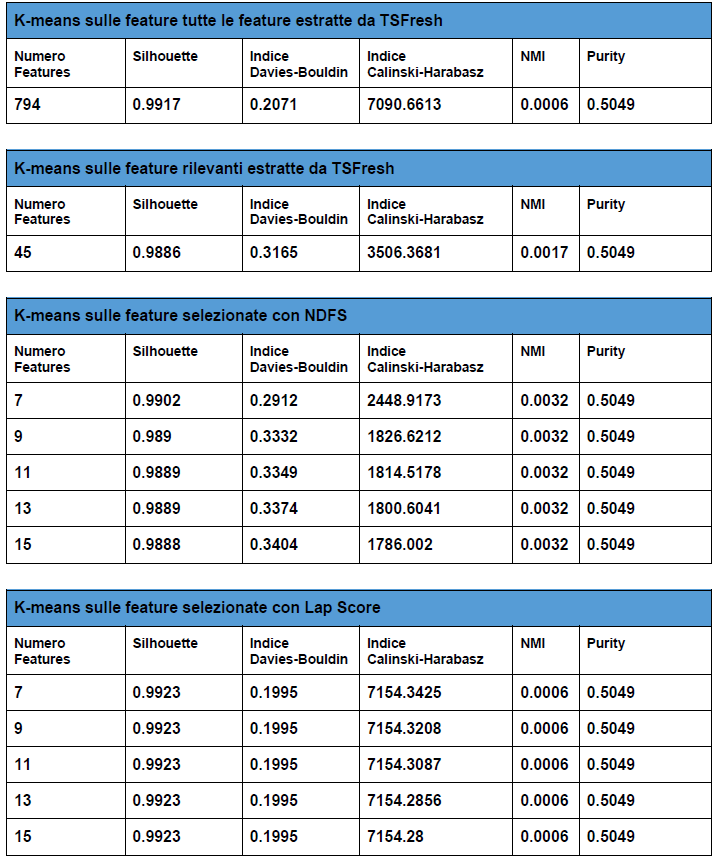
\includegraphics[width=0.9\linewidth]{av/fordb_av.png}
	\caption{FordB con tecniche di feature extraction and selection.\\
	\\
	\textbf{L'autoencoder ha silhouette e DB di gran lunga peggiori rispetto a quattro gli algoritmi}, mentre la purity è simile in tutti i casi. DB è quasi ottimale con Lap Score. E' una situazione simile a quella di FordA.}
	\label{fig:fordb_av}
\end{figure}

\subsubsection{PhalangesOutlineCorrect}
\begin{figure}[H]
	\centering
	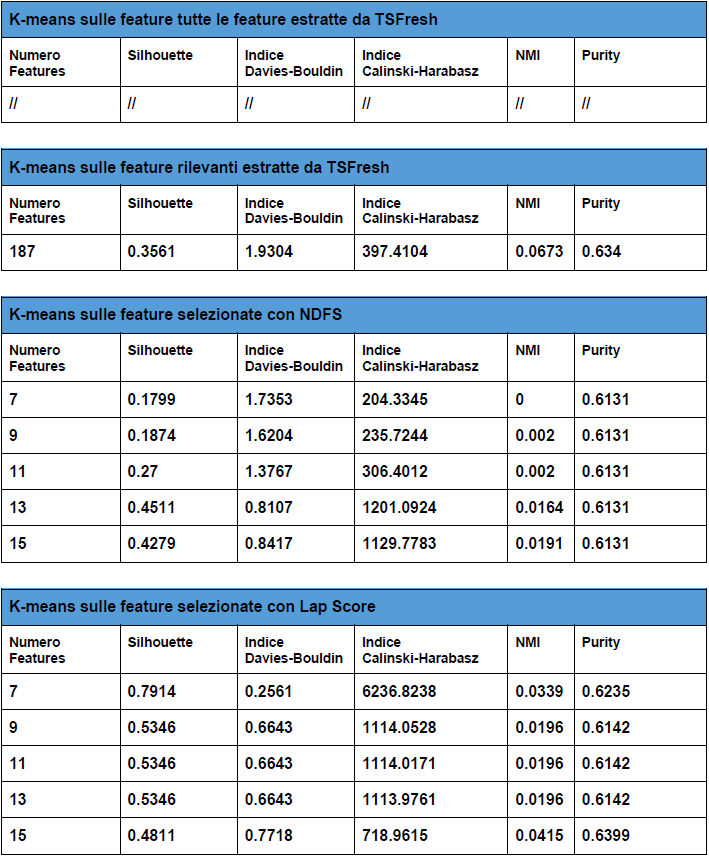
\includegraphics[width=0.9\linewidth]{av/phalanges_av.png}
	\caption{PhalangesOutlineCorrect con tecniche di feature extraction and selection.\\
	\\
	\textbf{L'autoencoder ha purity simile a tutti e quattro gli algoritmi}, mentre ha silhouette e DB variabili: migliori rispetto a TSFresh e una parte di NDFS, peggiori rispetto a Lap Score e un'altra parte di NDFS.}
	\label{fig:phalanges_av}
\end{figure}

\subsubsection{RefrigerationDevices}
\begin{figure}[H]
	\centering
	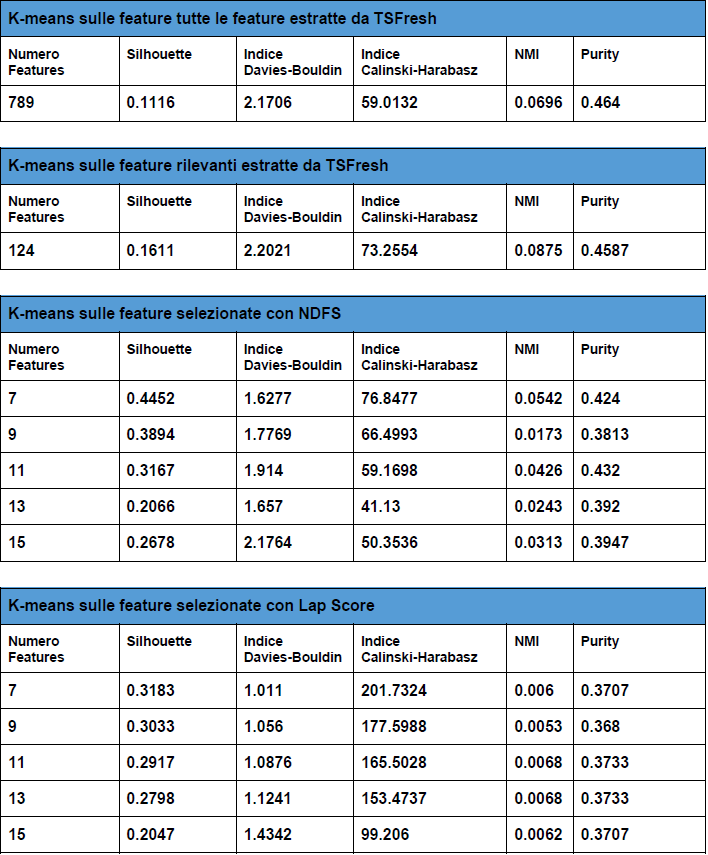
\includegraphics[width=0.9\linewidth]{av/refrigeration_av.png}
	\caption{RefrigerationDevices con tecniche di feature extraction and selection.\\
	\\
	\textbf{L'autoencoder ha purity simile a tutti e quattro gli algoritmi, a meno di leggere differenza}, mentre ha silhouette e DB ben peggiori rispetto a tutti gli algoritmi. In particolare, la silhouette migliora con NDFS e Lap Score.}
	\label{fig:refrigeration_av}
\end{figure}

\subsubsection{TwoLeadECG}
\begin{figure}[H]
	\centering
	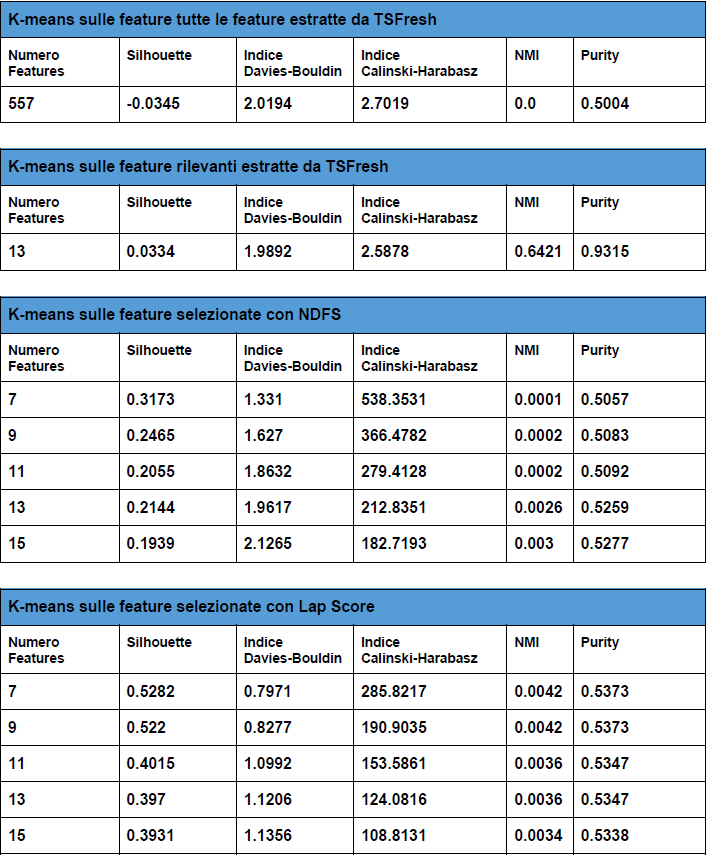
\includegraphics[width=0.9\linewidth]{av/twoleadecg_av.png}
	\caption{TwoLeadECG con tecniche di feature extraction and selection.\\
	\\
	\textbf{L'autoencoder ha silhouette e DB mediamente migliori di tutti e quattro gli algoritmi}, infatti ci sono alcune esecuzioni di Lap Score dove invece si ha una situazione ribaltata. La purity è simile in quasi tutti i casi.}
	\label{fig:twoleadecg_av}
\end{figure}

\subsubsection{TwoPatterns}
\begin{figure}[H]
	\centering
	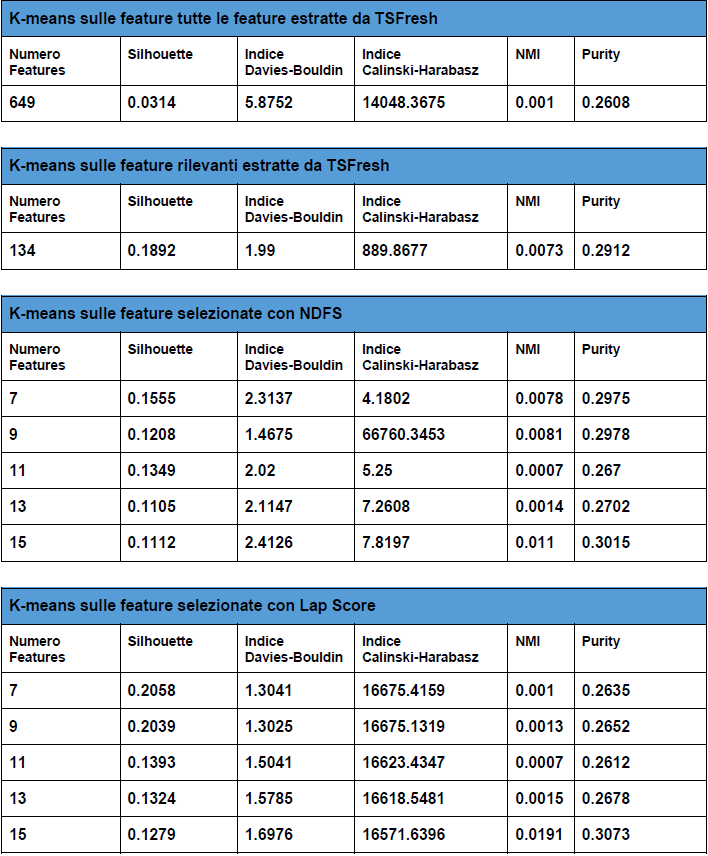
\includegraphics[width=0.9\linewidth]{av/twopatterns_av.png}
	\caption{TwoPatterns con tecniche di feature extraction and selection.\\
	\\
	\textbf{L'autoencoder ha silhouette e DB di gran lunga peggiori rispetto ai quattro algoritmi}, tuttavia la silhouette dei quattro algoritmi è comunque molto bassa. La purity è molto simile in tutti casi, sebbene anche essa risulti molto bassa.}
	\label{fig:twopatterns_av}
\end{figure}

\chapter{Conclusioni} \label{chap:conclusioni}
Con questo esperimento si è voluto valutare diverse tecniche di clustering su Time Series, andando a verificare come tecniche di feature extraction and selection potessero influenzare (sia in positivo che in negativo) i risultati dei clustering.
A tal fine si sono confrontate due diverse tecniche di feature extraction/selection (TSFresh ed autoencoder) e si sono confrontati con un clustering applicato su time series pure, mediante la dovuta metrica di distanza (k-Means con DTW di TSLearn).
I risultati ottenuti ci permettono di formulare varie considerazioni.\\ 
\\
Innanzitutto, \textbf{l'autoencoder si è mostrato particolarmenre efficace ad estrarre le principali caratteristiche dai dataset relativi agli elettrocardiogrammi}, ovvero ECG5000, ECG200 e TwoLeadECG.
Per i dataset "rumorosi", quali FordA, FordB, RefrigerationDevices e TwoPatterns, i risultati sono stati abbastanza scadenti: allo stato attuale, il nostro modello non è stato in grado di cogliere le caratteristiche di queste TS.
Gli altri dataset, ChlorineConcetration e PhalangesOutlineCorrect, hanno dato risultati buoni, ma migliorabili con alcune modifiche agli iperaparametri del modello.\\
\\
Tutte le tecniche hanno presentato \textbf{difficoltà nell'ottenere score interni alti per alcuni dataset}. Questo può essere causato dal fatto che alcuni dataset potrebbero essere densi, quindi molte TS risultano "vicine" nello spazio, andando a danneggiare compattezza e separazione dei cluster.\\
Inoltre, k-Means è un algoritmo che minimizza la varianza intra-cluster piuttosto che massimizzare la densità dei cluster, quindi gli score come Davies-Bouldin non sono sempre ottimali, essendo basati proprio sulla densità.\\
\\
Tutte le tecniche hanno riscontrato \textbf{dei limiti nella massimizzazione di score esterni per alcuni dataset}. Questo può essere causato dal fatto che alcuni dataset presentano classi fortemente sbilanciate, oppure classi con TS molto diverse tra loro, cosa che è stata notata durante la fase di data profiling.\\
\\
Si è verificato, inoltre, che per i vari clustering calcolati sui vettori latenti estratti dall'autoencoder, si ottenevano \textbf{misure di qualità interne migliori} per un\textbf{numero di cluster basso}, come due o tre, mentre per valori di cluster alti, come cinque o sei, esse peggioravano.
Tale andamento, seppur in maniera più ridotta, si è riscontrato anche per le misure esterne.\\
\\ 
In generale, gli score sono stati \textbf{utili per confrontare tra loro le diverse tecniche}, accomunate dall'algoritmo k-Means, \textbf{ma non sono significativi al fine di valutare la bontà in assoluto di una tecnica di clustering}.

\addcontentsline{toc}{chapter}{Bibliografia}
\printbibliography

\end{document}